\documentclass[twoside,12pt,notitlepage]{book}

\input macros

\begin{document}



\frontmatter
\input Upodgata
\bfseries
\thispagestyle{empty}
\fontsize{14}{16}\selectfont
\tableofcontents
\clearpage

\mainmatter

\renewcommand{\thepage}{\devanagarinumeral{page}}
\thispagestyle{empty}
\section[गुरुपादुकास्तोत्रम्]{अथ  गुरुपादुकास्तोत्रम्}

\noindent अनन्तसंसारसमुद्रतारनौकायिताभ्यां गुरुभक्तिदाभ्याम्~। \\[-6pt]
वैराग्यसाम्राज्यदपूजनाभ्यां नमो नमश्श्रीगुरुपादुकाभ्याम्~॥१॥\\
कवित्ववाराशिनिशाकराभ्यां दौर्भाग्यदावाम्बुदमालिकाभ्याम्~।\\[-6pt]
दूरीकृतानम्रविपत्ततिभ्यां नमो नमश्श्रीगुरुपादुकाभ्याम्~॥२॥\\
नता ययोः श्रीपतितां समीयुः कदाचिदप्याशु दरिद्रवर्याः~।\\[-6pt]
मूकाश्च वाचस्पतितां हि ताभ्यां नमो नमश्श्रीगुरुपादुकाभ्याम्~॥३॥\\
नालीकनीकाशपदाहृताभ्यां नानाविमोहादिनिवारिकाभ्यां~।\\[-6pt]
नमज्जनाभीष्टततिप्रदाभ्यां नमो नमश्श्रीगुरुपादुकाभ्याम्~॥४॥\\
नृपालिमौलिव्रजरत्नकान्तिसरिद्विराजज्झषकन्यकाभ्याम्~।\\[-6pt]
नृपत्वदाभ्यां नतलोकपङ्क्तेः नमो नमश्श्रीगुरुपादुकाभ्याम्~॥५॥\\
पापान्धकारार्कपरम्पराभ्यां तापत्रयाहीन्द्रखगेश्वराभ्याम्~।\\[-6pt]
जाड्याब्धिसंशोषणवाडवाभ्यां नमो नमश्श्रीगुरुपादुकाभ्याम्~॥६॥\\
शमादिषट्कप्रदवैभवाभ्यां समाधिदानव्रतदीक्षिताभ्याम्~।\\[-6pt]
रमाधवाङ्घ्रिस्थिरभक्तिदाभ्यां नमो नमश्श्रीगुरुपादुकाभ्याम्~॥७॥\\
स्वार्चापराणामखिलेष्टदाभ्यां स्वाहासहायाक्षधुरन्धराभ्याम्~।\\[-6pt]
स्वान्ताच्छभावप्रदपूजनाभ्यां नमो नमश्श्रीगुरुपादुकाभ्याम्~॥८॥\\
कामादिसर्पव्रजगारुडाभ्यां विवेकवैराग्यनिधिप्रदाभ्याम्~।\\[-6pt]
बोधप्रदाभ्यां द्रुतमोक्षदाभ्यां नमो नमश्श्रीगुरुपादुकाभ्याम्~॥९॥

\noindent {\small ॥~इति श्रीसच्चिदानन्दशिवाभिनवनृसिंहभारतीस्वामिभिः विरचितं गुरुपादुकास्तोत्रम्~॥}

\clearpage
\section[गुर्वष्टकम्]{ गुर्वष्टकम्}
\noindent शरीरं सुरूपं तथा वा कलत्रं यशश्चारु चित्रं धनं मेरुतुल्यम्~।\\[-6pt]
मनश्चेन्न लग्नं गुरोरङ्घ्रिपद्मे ततः किं ततः किं ततः किं ततः किम्~॥१॥\\
कलत्रं धनं पुत्रपौत्रादि सर्वं गृहं बान्धवाः सर्वमेतद्धि जातम्~।\\[-6pt]
मनश्चेन्न लग्नं गुरोरङ्घ्रिपद्मे ततः किं ततः किं ततः किं ततः किम्~॥२॥\\
षडङ्गादिवेदो मुखे शास्त्रविद्या कवित्वादि गद्यं सुपद्यं करोति~।\\[-6pt]
मनश्चेन्न लग्नं गुरोरङ्घ्रिपद्मे ततः किं ततः किं ततः किं ततः किम्~॥३॥\\
विदेशेषु मान्यः स्वदेशेषु धन्यः सदाचारवृत्तेषु मत्तो न चान्यः~।\\[-6pt]
मनश्चेन्न लग्नं गुरोरङ्घ्रिपद्मे ततः किं ततः किं ततः किं ततः किम्~॥४॥\\
क्षमामण्डले भूपभूपालवृन्दैः सदा सेवितं यस्य पादारविन्दम्~।\\[-6pt]
मनश्चेन्न लग्नं गुरोरङ्घ्रिपद्मे ततः किं ततः किं ततः किं ततः किम्~॥५॥\\
यशो मे गतं दिक्षु दानप्रतापाज्जगद्वस्तु सर्वं करे यत्प्रसादात्~।\\[-6pt]
मनश्चेन्न लग्नं गुरोरङ्घ्रिपद्मे ततः किं ततः किं ततः किं ततः किम्~॥६॥\\
न भोगे न योगे न वा वाजिराजौ न कान्तामुखे नैव वित्तेषु चित्तम्~।\\[-6pt]
मनश्चेन्न लग्नं गुरोरङ्घ्रिपद्मे ततः किं ततः किं ततः किं ततः किम्~॥७॥\\
अरण्ये न वा स्वस्य गेहे न कार्ये न देहे मनो वर्तते मे त्वनर्घ्ये~।\\[-6pt]
मनश्चेन्न लग्नं गुरोरङ्घ्रिपद्मे ततः किं ततः किं ततः किं ततः किम्~॥८॥\\
गुरोरष्टकं यः पठेत्पुण्यदेही यतिर्भूपतिर्ब्रह्मचारी च गेही~।\\[-6pt]
लभेद्वाञ्छितार्थं पदं ब्रह्मसंज्ञं गुरोरुक्तवाक्ये मनो यस्य लग्नम्~॥९॥

\hfil {\small ॥~इति श्रीशङ्करभगवत्पादविरचितं गुर्वष्टकम्~॥}

\thispagestyle{empty}

\clearpage
\section{गुरुगीता}
\begin{verse}[\versewidth]
हंसाभ्यां परिवृत्तहार्दकमले शुद्धे जगत्कारणं\\[-6pt]
विश्वाकारमनेकदेहनिलयं स्वच्छन्दमानन्दकम्~।\\[-6pt]
सर्वाधारमखण्डचिद्घनरसं पूर्णं ह्यनन्तं शुभं\\[-6pt]
प्रत्यक्षाक्षरविग्रहं गुरुवरं ध्यायेद्विभुं शाश्वतम्~॥\\
नमामि सद्गुरुं शान्तं प्रत्यक्षं शिवरूपिणम्~।\\[-6pt]
शिरसा योगपीठस्थं मुक्तिकाम्यार्थसिद्धये~॥\\
ऋषय ऊचुः –\\
गुह्यात् गुह्यतरा सारा गुरुगीता विशेषतः~।\\[-6pt]
तव प्रसादाच्छ्रोतव्या तां सर्वां ब्रूहि सूत नः~॥१॥\\
सूत उवाच –\\
कैलासशिखरे रम्ये भक्तानुग्रहतत्परम्~।\\[-6pt]
प्रणम्य पार्वती भक्त्या शङ्करं परिपृच्छति~॥२॥\\
पार्वत्युवाच –\\
नमस्ते देवदेवेश परात्पर जगद्गुरो~।\\[-6pt]
सदाशिव महादेव गुरुदीक्षां प्रयच्छ मे~॥३॥\\
भगवन् सर्वधर्मज्ञ व्रतानामुत्तमोत्तमम्~।\\[-6pt]
ब्रूहि मे कृपया शम्भो गुरुमाहात्म्यमद्भुतम्~॥४॥\\
केन मार्गेण भो स्वामिन् देही ब्रह्ममयो भवेत्~।\\[-6pt]
कुरु मेऽनुग्रहं देव नमामि चरणौ तव~॥५॥\\
ईश्वर उवाच – \\
मम रूपासि देवि त्वं त्वद्भक्त्या तद्वदाम्यहम्~।\\[-6pt]
लोकोपकारकः प्रश्नः कृतः केनापि नो पुरा~॥६॥\\
यो गुरुः स शिवः प्रोक्तो यः शिवः स गुरुः स्मृतः~।\\[-6pt]
विकल्पं यस्तु कुर्वीत स भवेत् पातकी गुरौ~॥७॥\\
दुर्लभं त्रिषु लोकेषु तच्छृणु प्रवदाम्यहम्~।\\[-6pt]
गुरुं ब्रह्म विना नान्यत् सत्यं सत्यं वरानने~॥८॥\\
वेदशास्त्रपुराणानि सेतिहासादिकानि च~।\\[-6pt]
मन्त्रतन्त्रादिविद्याश्च स्मृतिरुच्चाटनादिकम्~॥९॥\\
शैवशाक्तागमादीनि ह्यन्ये च बहवो मताः~।\\[-6pt]
भ्रामकाः सर्व एवैते जीवानामल्पचेतसाम्~॥१०॥\\
यज्ञो व्रतं तपो दानं जपस्तीर्थं तथैव च~।\\[-6pt]
सर्वेषामेव जन्तूनां सर्वे मार्गाः प्रतारकाः~॥११॥\\
जपस्तपो व्रतं तीर्थं यज्ञो दानं तथैव च~।\\[-6pt]
गुरुतत्त्वमविज्ञाय सर्वं व्यर्थं भवेत्प्रिये~॥१२॥\\
गुरोर्विद्यात्मनो नान्यत् सत्यं सत्यं न संशयः~।\\[-6pt]
तल्लाभार्थं प्रयत्नस्तु कर्तव्यो हि मनीषिभिः~॥१३॥\\
रूढाविद्या जगन्माया देहेस्ति ध्वान्तरूपणी~।\\[-6pt]
तद्वारकः प्रकाशश्च गुरुशब्देन कथ्यते~॥१४॥\\
यदङ्घ्रिकमलद्वन्द्वं द्वन्द्वतापनिवारकम्~।\\[-6pt]
तारकं भवसिन्धोश्च तं गुरुं प्रणमाम्यहम्~॥१५॥\\
देही ब्रह्म भवेद्यस्मात् तदिदानीं प्रकाशये~।\\[-6pt]
सर्वपापविशुद्धात्मा श्रीगुरोः पादसेवनम्~॥१६॥\\
गुरोः पादोदकं पीत्वा धृत्वा शिरसि पावनम्~।\\[-6pt]
सर्वतीर्थावगाहस्य सम्प्राप्नोति फलं नरः~॥१७॥\\
शोषणं पापपङ्कस्य दीपनं ज्ञानतेजसः~।\\[-6pt]
गुरोः पादोदकं देवि संसारार्णवतारकम्~॥१८॥\\
अविद्यामूलनाशाय जन्मकर्मनिवृत्तये~।\\[-6pt]
ज्ञानवैराग्यसिद्ध्यर्थं गुरुपादोदकं पिबेत्~॥१९॥\\
गुरुपादोदकं पानं गुरोरुच्छिष्टभोजनम्~।\\[-6pt]
गुरुमूर्तेः सदाध्यानं गुरुस्तोत्रं परो जपः~॥२०॥\\
स्वदेशिकस्यैव च नामकीर्तनं\\[-6pt] भवेदनन्तस्य शिवस्य कीर्तनम्~।\\[-6pt]
स्वदेशिकस्यैव च रूपचिन्तनं\\[-6pt] भवेदनन्तस्य शिवस्य चिन्तनम्~॥२१॥\\
यत्पादपांसवः सन्तः केऽपि संसारवारिधेः~।\\[-6pt]
सेतुबन्धाय कल्पन्ते देशिकं तमुपास्महे~॥२२॥\\
काशीक्षेत्रं निवासश्च जाह्नवी चरणोदकम्~।\\[-6pt]
गुरुर्विश्वेश्वरः साक्षात् तारकं ब्रह्म निश्चितम्~॥२३॥\\
गुरोः पादाङ्कितं यत्र गया साऽधोक्षजोद्भवा~।\\[-6pt]
तीर्थराजः प्रयागोऽसौ गुरुमूर्त्यै नमो नमः~॥२४॥\\
गुरुमूर्तिं स्मरेन्नित्यं गुरोर्नाम सदा जपेत्~।\\[-6pt]
गुरोराज्ञां प्रकुर्वीत गुरोरन्यं न भावयेत्~॥२५॥\\
गुरुवक्त्रे स्थिता  विद्या प्राप्यते तत्प्रसादतः~।\\[-6pt]
तस्मात्तं देशिकं ध्यायेद्यथा योषित्प्रियं स्वकम्~॥२६॥\\
स्वाश्रमं च स्वजातिं च स्वकीर्तिं पुष्टिवर्धनम्~।\\[-6pt]
एतत्सर्वं परित्यज्य गुरुमेव समाश्रयेत्~॥२७॥\\
अनन्याश्चिन्तयन्तो ये ध्रुवं तेषां परं पदम्~।\\[-6pt]
तस्मात्सर्वप्रयत्नेन गुरोराराधनं कुरु~॥२८॥\\
गुरोर्मुखाच्च सम्प्राप्य देवि ब्रह्मात्मसंविदम्~।\\[-6pt]
त्रैलोक्यस्फुटवक्तारो देवर्षिपितृमानवाः~॥२९॥\\
गुकारश्चान्धकारो हि रुकारस्तेज उच्यते~।\\[-6pt]
अज्ञानग्रासकं ब्रह्म गुरुरेव न संशयः~॥३०॥\\
गुकारश्चान्धकारस्तु रुकारस्तन्निरोधकः~।\\[-6pt]
अन्धकारविनाशित्वात् गुरुरित्यभिधीयते~॥३१॥\\
गुकारः स्याद्गुणातीतो रूपातीतो रुकारकः~।\\[-6pt]
गुणरूपविहीनत्वाद्गुरुरित्यभिधीयते~॥३२॥\\
गुकारः प्रथमो वर्णो मायादिगुणभासकः~।\\[-6pt]
रुकारोऽस्ति परं ब्रह्म  मायाभ्रान्तिविमोचकम्~॥३३॥\\
एवं गुरुपदं श्रेष्ठं देवानामपि दुर्लभम्~।\\[-6pt]
हाहाहूहूगणैश्चैव गन्धर्वैरपि पूजितम्~॥३४॥\\
ध्रुवं तेषां च सर्वेषां नास्ति तत्त्वं गुरोः परम्~।\\[-6pt]
गुरोराराधानं कार्यं स्वजीवत्वं निवेदयेत्~॥३५॥\\
आसनं शयनं वस्त्रं वाहनं भूषणादिकम्~।\\[-6pt]
साधकेन प्रदातव्यं गुरोः सन्तोषकारणम्~॥३६॥\\
कर्मणा मनसा वाचा नित्यमाराधयेद्गुरुम्~।\\[-6pt]
दीर्घदण्डं नमस्कुर्यान्निर्लज्जो गुरुसन्निधौ~॥३७॥\\
शरीरमर्थं प्राणांश्च सद्गुरुभ्यो निवेदयेत्~।\\[-6pt]
आत्मानमपि दास्याय वैदेहो जनको यथा~॥३८॥\\
गुरुरेव जगत्सर्वं ब्रह्मविष्णुशिवात्मकम्~।\\[-6pt]
गुरोः परतरं नास्ति तस्मात्तं पूजयेद्गुरुम्~॥३९॥\\
यस्यानुग्रहमात्रेण हृदि ह्युत्पद्यते क्षणात्~।\\[-6pt]
ज्ञानं च परमानन्दः सद्गुरुः शिव एव सः~॥४०॥\\
भस्मकीटविडं तं हि देहं स्थूलं वरानने~।\\[-6pt]
त्वङ्‍मूत्ररुधिरास्थीनि मलमांसादिभाजनम्~॥४१॥\\
संसारवृक्षमारूढाः पतन्तो नरकार्णवे~।\\[-6pt]
सर्वे येनोद्धृता लोकास्तस्मै श्रीगुरवे नमः~॥४२॥\\
गुरुर्ब्रह्मा गुरुर्विष्णुर्गुरुर्देवो महेश्वरः~।\\[-6pt]
गुरुरेव परं ब्रह्म तस्मै श्रीगुरवे नमः~॥४३॥\\
अखण्डमण्डलाकारं व्याप्तं येन चराचरम्~।\\[-6pt]
तत्पदं दर्शितं येन तस्मै श्रीगुरवे नमः~॥४४॥\\
देहे जीवत्वमापन्नं चैतन्यं निष्कलं परम्~।\\[-6pt]
त्वंपदं दर्शितं येन तस्मै श्रीगुरवे नमः~॥४५॥\\
अखण्डं परमार्थं सत् ऐक्यं च त्वंतदोः शुभम्~।\\[-6pt]
असिना दर्शितं येन तस्मै श्रीगुरवे नमः~॥४६॥\\
सर्वश्रुतिशिरोरत्ननीराजितपदाम्बुजम्~।\\[-6pt]
वेदान्ताम्बुजसूर्याभं श्रीगुरुं शरणं व्रजेत्~॥४७॥\\
चैतन्यं शाश्वतं शान्तं मायातीतं निरञ्जनम्~।\\[-6pt]
नादबिन्दुकलातीतं तस्मै श्रीगुरवे नमः~॥४८॥\\
स्थावरं जङ्गमं चेति यत्किञ्चिज्जगतीतले~।\\[-6pt]
व्याप्तं यस्य चिता सर्वं तस्मै श्रीगुरवे नमः~॥४९॥\\
त्वं पिता त्वञ्च मे माता त्वं बन्धुस्त्वं च दैवतम्~।\\[-6pt]
संसारप्रीतिभङ्गाय तुभ्यं श्रीगुरवे नमः~॥५०॥\\
यत्सत्तया जगत्सत्त्वं यत्प्रकाशेन भायुतम्~।\\[-6pt]
नन्दनं च यदानन्दात्तस्मै श्रीगुरवे नमः~॥५१॥\\
येन चेतयताऽऽपूर्य चित्तं चेतयते नरः~।\\[-6pt]
जाग्रत्स्वप्नसुषुप्त्यादौ तस्मै श्रीगुरवे नमः~॥५२॥\\
यस्य ज्ञानादिदं विश्वमदृश्यं भेदभेदतः~।\\[-6pt]
सत्स्वरूपावशेषञ्च तस्मै श्रीगुरवे नमः~॥५३॥\\
य एव कार्यरूपेण कारणेनापि भाति च~।\\[-6pt]
कार्यकारणनिर्मुक्तस्तस्मै श्रीगुरवे नमः~॥५४॥\\
ज्ञानशक्तिस्वरूपाय कामितार्थप्रदायिने~।\\[-6pt]
भुक्तिमुक्तिप्रदात्रे च तस्मै श्रीगुरवे नमः~॥५५॥\\
अनेकजन्मसम्प्राप्तकर्मकोटिविदाहिने~।\\[-6pt]
ज्ञानानलप्रभावेन तस्मै श्रीगुरवे नमः~॥५६॥\\
न गुरोरधिकं तत्त्वं न गुरोरधिकं तपः~।\\[-6pt]
न गुरोरधिकं ज्ञानं तस्मै श्रीगुरवे नमः~॥५७॥\\
मन्नाथः श्रीजगन्नाथो मद्गुरुः श्रीजगद्गुरुः~।\\[-6pt]
ममात्मा सर्वभूतात्मा तस्मै श्रीगुरवे नमः~॥५८॥\\
गुरुरादिरनादिश्च गुरुः परमदैवतम्~।\\[-6pt]
गुरोः समानः को वास्ति तस्मै श्रीगुरवे नमः~॥५९॥\\
एक एव परो बन्धुर्विषमे समुपस्थिते~।\\[-6pt]
निस्स्पृहः करुणासिन्धुस्तस्मै श्रीगुरवे नमः~॥६०॥\\
गुरुमध्ये स्थितं विश्वं विश्वमध्ये स्थितो गुरुः~।\\[-6pt]
विश्वरूपो विरूपोऽसौ तस्मै श्रीगुरवे नमः~॥६१॥\\
भवारण्यप्रविष्टस्य दिङ्‍मोहभ्रान्तचेतसः~।\\[-6pt]
येन सन्दर्शितः पन्थास्तस्मै श्रीगुरवे नमः~॥६२॥\\
तापत्रयाग्नितप्तानां श्रान्तानां प्राणिनाम् उमे~।\\[-6pt]
गुरुरेव परा गङ्गा तस्मै श्रीगुरवे नमः~॥६३॥\\
हेतवे सर्वजगतां संसारार्णवसेतवे~।\\[-6pt]
प्रभवे सर्वविद्यानां शम्भवे गुरवे नमः~॥६४॥\\
ध्यानमूलं गुरोर्मूर्तिः पूजामूलं गुरोः पदम्~।\\[-6pt]
मन्त्रमूलं गुरोर्वाक्यं मोक्षमूलं गुरोः कृपा~॥६५॥\\
हरणं भवरोगस्य तरणं क्लेशवारिधेः ~।\\[-6pt]
भरणं सर्वलोकस्य शरणं चरणं गुरोः~॥६६॥\\
शिवे रुष्टे गुरुस्त्राता गुरौ रुष्टे न कश्चन~।\\[-6pt]
तस्मात् परगुरुं लब्ध्वा तमेव शरणं व्रजेत्~॥६७॥\\
अत्रिणेत्रः शिवः साक्षात् द्विभुजश्चापरो हरिः~।\\[-6pt]
योऽचतुर्वदनो ब्रह्मा श्रीगुरुः कथितः प्रिये~॥६८॥\\
नित्याय निर्विकाराय निरवद्याय योगिने~।\\[-6pt]
निष्कलाय निरीहाय शिवाय गुरवे नमः~॥६९॥\\
शिष्यहृत्पद्मसूर्याय सत्याय ज्ञानस्वरूपिणे~।\\[-6pt]
वेदान्तवाक्यवेद्याय शिवाय गुरवे नमः~॥७०॥\\
उपायोपेयरूपाय सदुपायप्रदर्शिने~।\\[-6pt]
अनिर्वाच्याय वाच्याय शिवाय गुरवे नमः~॥७१॥\\
कार्यकारणरूपाय रूपारूपाय ते सदा~।\\[-6pt]
अप्रमेयस्वरूपाय शिवाय गुरवे नमः~॥७२॥\\
दृग्दृश्यद्रष्टृरूपाय निष्पन्ननिजरूपिणे~।\\[-6pt]
अपारायाद्वितीयाय शिवाय गुरवे नमः~॥७३॥\\
गुणाधाराय गुणिने गुणरूपस्वरूपिणे~।\\[-6pt]
जन्मिने जन्महीनाय शिवाय गुरवे नमः~॥७४॥\\
अनाद्यायाखिलाद्याय मायिने गतमायिने~।\\[-6pt]
अरूपाय स्वरूपाय शिवाय गुरवे नमः~॥७५॥\\
सर्वमन्त्रस्वरूपाय सर्वतन्त्रस्वरूपिणे~।\\[-6pt]
सर्वगाय समस्ताय शिवाय गुरवे नमः~॥७६॥\\
श्रीनाथचरणद्वन्द्वं यस्यां दिशि विराजते~।\\[-6pt]
तस्यै दिशे नमस्कुर्यात्  भक्त्या प्रतिदिनं प्रिये~॥७९॥\\
तस्यै दिशे सततमञ्जलिरेष नित्यं\\
प्रक्षिप्यते मुखरितालियुतप्रसूनैः~।\\[-6pt]
जागर्ति यत्र भगवान् गुरुचक्रवर्ती\\
विश्वस्थितिप्रलयनाटकविश्वसाक्षी~॥८०॥\\
उरसा शिरसा चैव मनसा वचसा दृशा~।\\[-6pt]
पद्‍भ्यां कराभ्यां कर्णाभ्यां प्रणामोऽष्टाङ्ग उच्यते~॥८१॥\\
गुरोः कृपाप्रसादेन ब्रह्मविष्णुमहेश्वराः~।\\[-6pt]
समर्थास्तत्प्रसादो हि केवलं गुरुसेवया~॥८२॥\\
देवकिन्नरगन्धर्वाः पितरो यक्षचारणाः~।\\[-6pt]
मुनयो नैव जानन्ति गुरुशुश्रूषणे विधिम्~॥८३॥\\
मदाहङ्कारगर्वेण तपोविद्याबलान्विताः~।\\[-6pt]
संसारकुहरावर्ते पतिता घटयन्त्रवत्~॥८४॥\\
ध्यानं श्रुणु महादेवि श्रीगुरोः कथयामि ते~।\\[-6pt]
सर्वसौख्यकरं तद्वद्भुक्तिमुक्तिप्रदायकम्~॥८५॥\\
श्रीमत्परब्रह्मगुरुं स्मरामि श्रीमत्परब्रह्मगुरुं भजामि~।\\[-6pt]
श्रीमत्परब्रह्मगुरुं वदामि श्रीमत्परब्रह्मगुरुं नमामि~॥८६॥\\
ब्रह्मानन्दं परमसुखदं केवलं ज्ञानमूर्तिं\\[-6pt]
द्वन्द्वातीतं गगनसदृशं तत्त्वमस्यादिलक्ष्यम्~।\\[-6pt]
एकं नित्यं विमलमचलं सर्वधीसाक्षिभूतं\\[-6pt]
भावातीतं त्रिगुणरहितं सद्गुरुं तं नमामि~॥८७॥\\
आनन्दमानन्दकरं प्रसन्नं\\[-6pt]
ज्ञानस्वरूपं निजबोधयुक्तम्~।\\[-6pt]
योगीन्द्रमीड्यं भवरोगवैद्यं\\[-6pt]
श्रीमद्गुरुं नित्यमहं नमामि~॥८८॥\\
नित्यं शुद्धं निराभासं निराकारं निरञ्जनम्~।\\[-6pt]
नित्यबोधचिदानन्दं गुरुं ब्रह्म नमाम्यहम्~॥८९॥\\
हृदम्बुजे कर्णिकमध्यसंस्थे\\[-6pt]
सिंहासने संस्थितदिव्यमूर्तिम्~।\\[-6pt]
ध्यायेद्गुरुं चन्द्रकलाप्रकाशं\\[-6pt]
सच्चित्सुखाभीष्टवरं ददानम्~॥९०॥\\
श्वेताम्बरं श्वेतविलेपपुष्पं\\[-6pt]
मुक्ताविभूषं मुदितं त्रिणेत्रम्~।\\[-6pt]
वामाङ्कपीठस्थितदिव्यशक्तिं\\[-6pt]
मन्दस्मितं सान्द्रकृपानिधानम्~॥९१॥\\
यस्मिन् सृष्टिस्थितिध्वंसनिग्रहानुग्रहात्मकम्~।\\[-6pt]
कृत्यं पञ्चविधं शश्वद्भासते तं गुरुं भजेत्~॥९२॥\\
न गुरोरधिकं न गुरोरधिकं\\[-6pt]
न गुरोरधिकं न गुरोरधिकं~।\\[-6pt]
शिवशासनतः शिवशासनतः\\[-6pt]
शिवशासनतः शिवशासनतः~॥९३~॥\\
ज्ञेयं सर्वं विलाप्येत विशुद्धज्ञानयोगतः~।\\[-6pt]
ज्ञातृत्वमपि चिन्मात्रे नान्यः पन्था द्वितीयकः~॥९४॥\\
यावत्तिष्ठति देहेऽसौ तावद्देवि गुरुं स्मरेत्~।\\[-6pt]
गुरुलोपो न कर्तव्यो निष्ठितोप्यद्वये परे~॥९५॥\\
हुंकारेण न वक्तव्यं प्राज्ञैः शिष्यैः कदाचन~।\\[-6pt]
गुरोरग्रे न वक्तव्यमसत्यं च कदाचन~॥९६॥\\ 
गुरुं त्वंकृत्य हुंकृत्य गुरुं निर्जित्य वादतः~।\\[-6pt]
अरण्ये निर्जले घोरे स भवेद् ‍ब्रह्मराक्षसः~॥९७॥\\
उपभुञ्जीत नो वस्तु गुरोः किञ्चिदपि स्वयम्~।\\[-6pt]
दत्तं ग्राह्यं  प्रसादेति प्रायो ह्येतन्न लभ्यते~॥९८॥\\
पादुकासनशय्यादि गुरुणा यदधिष्ठितम्~।\\[-6pt]
नमस्कुर्वीत तत्सर्वं पादाभ्यां न स्पृशेत्क्वचित्~॥९९॥\\
गच्छतः पृष्ठतो गच्छेत् गुरुपादौ न लङ्घयेत्~।\\[-6pt]
नोल्बणं धारयेद्वेषं नालाङ्कारांस्तथोल्बणान्~॥१००॥\\
गुरुनिन्दापरं दृष्ट्वा धावयेदथ वारयेत्~।\\[-6pt]
स्थानं वा तत् परित्याज्यं जिह्वाच्छेदाऽक्षमो यदि~॥१०१॥\\
अप्रियस्य च हास्यस्य नावकाशो गुरोः पुरः~।\\[-6pt]
न नियोगपरं ब्रूयात् गुरोराज्ञां विभावयेत्~॥१०२॥\\
मुनिभ्यः पन्नगेभ्यश्च सुरेभ्यः शापतोऽपि च~।\\[-6pt]
कालमृत्युभयाद्वापि गुरू रक्षति पार्वति~॥१०३॥\\
नित्यं ब्रह्म निराकारं येन प्राप्तं स वै गुरुः~।\\[-6pt]
स शिष्यं प्रापयेत् प्राप्यं दीपो दीपान्तरं यथा~॥१०४॥\\
गुरोः कृपाप्रसादेन ब्रह्माहमिति भावयेत्~।\\[-6pt]
अनेन मुक्तिमार्गेण ह्यात्मज्ञानं प्रकाशते~॥१०५॥\\
संपश्येच्छ्रीगुरुं शान्तं परमात्मस्वरूपिणम्~।\\[-6pt]
स्थावरे जङ्गमे चैव सर्वत्र जगतीतले~॥१०६॥\\
श्रीगुरुं सच्चिदानन्दं भावातीतं विभाव्य च~।\\[-6pt]
तन्निदर्शितमार्गेण ध्यानमग्नो भवेत्सुधीः~॥१०७॥\\
परात्परतरं ध्यायेच्छुद्धस्फटिकसन्निभम्~।\\[-6pt]
हृदयाकाशमध्यस्थं स्वाङ्गुष्ठपरिमाणकम्~॥१०८॥\\
अङ्गुष्ठमात्रं पुरुषं ध्यायतश्चिन्मयं हृदि~।\\[-6pt]
तत्र स्फुरति यो भावः शृणु तत्कथयामि ते~॥१०९॥\\
विरजं परमाकाशं  ध्रुवमानन्दमव्ययम्~।\\[-6pt]
	अगोचरं तथाऽऽगम्यं नामरूपविवर्जितम्~॥११०॥\\
	तदहं ब्रह्म कैवल्यमिति बोधः प्रजायते~।\\[-6pt]
यथा निजस्वभावेन केयूरकटकादयः~।\\[-6pt]
सुवर्णत्वेन तिष्ठन्ति तथाऽहं ब्रह्म शाश्वतम्~॥१११॥\\
एवं ध्यायन् परं ब्रह्म स्थातव्यं यत्र कुत्रचित्~।\\[-6pt]
कीटो भृङ्ग इव ध्यानात् ब्रह्मैव भवति स्वयम्~॥११२॥\\
यदृच्छया चोपपन्नं ह्यल्पं बहुळमेव वा~।\\[-6pt]
नीरागेणैव भुञ्जीत स्वाभ्याससमये मुदा~॥११३॥\\
एकमेवाद्वितीयोऽहं गुरुवाक्यात्सुनिश्चितम्~।\\[-6pt]
एवमभ्यस्यतो नित्यं न सेव्यं वै वनान्तरम्~॥११४॥\\
अभ्यासान्निमिषेणैव समाधिमधिगच्छति~।\\[-6pt]
जन्मकोटिकृतं पापं तत्क्षणादेव नश्यति~॥११५॥\\
न तत्सुखं सुरेन्द्रस्य न सुखं चक्रवर्तिनाम्~।\\[-6pt]
यत्सुखं वीतरागस्य सदा सन्तुष्टचेतसः~॥११६॥\\
रसं ब्रह्म पिबेद्यश्च तृप्तो यः परमात्मनि~।\\[-6pt]
इन्द्रं च मनुते रङ्कं नृपाणां तत्र का कथा~॥११७॥\\
देशः पूतो जनाः पूतास्तादृशो यत्र तिष्ठति~।\\[-6pt]
तत्कटाक्षोऽथ संसर्गः परस्मै श्रेयसेप्यलम्~॥११८॥\\
देही ब्रह्म भवेदेवं प्रसादाद्ध्यानतो गुरोः~।\\[-6pt]
नराणां च फलप्राप्तौ भक्तिरेव हि कारणम्~॥११९॥\\
मुक्तस्य लक्षणं देवि तवाग्रे कथितं मया~।\\[-6pt]
गुरुभक्तिस्तथा ध्यानं सकलं तव कीर्तनम्~॥१२०॥\\
गुरुगीतातिगुह्येयं मयाऽस्ति कथिता शुभा~।\\[-6pt]
श्रीगुरुं चिन्मयं ध्यायन् यामहं कलये सदा~॥१२१॥\\
गुरुगीतामिमां देवि शुद्धतत्त्वं मयोदितम्~।\\[-6pt]
गुरुं मां ध्यायती प्रेम्णा हृदि नित्यं विभावय~॥१२२॥\\
इयं चेद्भक्तिभावेन पठ्यते श्रूयतेऽथवा~।\\[-6pt]
लिख्यते दीयते पुम्भिर्भवेद्भवविनाशिनी~॥१२३॥\\
अनन्तफलमाप्नोति गुरुगीताजपेन तु~।\\[-6pt]
अस्याश्च विविधा मन्त्राः कलां नार्हन्ति षोडशीम्~॥१२४॥\\
सर्वपापप्रशमनी सर्वसङ्कटनाशिनी~।\\[-6pt]
सर्वसिद्धिकरी चेयं सर्वलोकवशङ्करी~॥१२५॥\\
दुःस्वप्ननाशिनी चेयं सुस्वप्नफलदायिनी~।\\[-6pt]
रिपूणां स्तम्भनी गीता वाचस्पत्यप्रदायिनी~॥१२६॥\\
कामिनां कामधेनुश्च सर्वमङ्गलकारिणी~।\\[-6pt]
चिन्तामणिश्चिन्तितस्य श्लोके श्लोके च सिद्धिदा~॥१२७॥\\
मोक्षकामो जपेन्नित्यं मोक्षश्रियमवाप्नुयात्~।\\[-6pt]
पुत्रकामो लभेत्पुत्रान् श्रीकामश्चामितां श्रियम्~॥१२८॥\\
त्रिवारपठनात्सद्यः कारागाराद्विमुच्यते~।\\[-6pt]
नित्यपाठाद्भवेच्च स्त्री पुत्रिणी सुभगा चिरम्~॥१२९॥\\
अकामतः स्त्री विधवा जपेन्मोक्षमवाप्नुयात्~।\\[-6pt]
अवैधव्यं सकामा चेल्ल्भते चान्यजन्मनि~॥१३०॥\\
जपेच्छाक्तश्च सौरश्च गाणपत्यश्च वैष्णवः~।\\[-6pt]
शैवश्च सिद्धिदामेतां सर्वदेवस्वरूपिणीम्~॥१३१॥\\
तीर्थे बिल्वतरोर्मूले वटमूले सरित्तटे~।\\[-6pt]
देवालये च गोष्ठे च मठे बृन्दावने तथा~।\\[-6pt]
पवित्रे निर्मले स्थाने जपः शीघ्रफलप्रदः~॥१३२॥\\
शान्त्यर्थे धारयेच्छुक्लं वस्त्रं वश्येऽथ रक्तिमम्~।\\[-6pt]
आभिचारे नीलवर्णं पीतवर्णं धनागमे~॥१३३॥\\
गुरुभक्तो भवेच्छीघ्रं गुरुगीताजपेन तु~।\\[-6pt]
धन्या माता पिता धन्यो धन्या वंश्या जना अपि~।\\[-6pt]
धन्या च वसुधा यत्र गुरुभक्तः प्रजायते~॥१३४॥\\
इदं रहस्यं नो वाच्यं यस्मै कस्मैचन प्रिये~।\\[-6pt]
अभक्ते वञ्चके धूर्ते पाषण्डे नास्तिके तथा~।\\[-6pt]
मनसाऽपि न वक्तव्या गुरुगीता कदाचन~॥१३५॥\\
अत्यन्तपक्वचित्तस्य श्रद्धाभक्तियुतस्य च~।\\[-6pt]
प्रवक्तव्या प्रयत्नेन ममात्मा प्रीयते तदा~॥१३६॥\\
गुरवो बहवः सन्ति शिष्यवित्तापहारकाः~।\\[-6pt]
दुर्लभः स गुरुर्लोके शिष्यसन्तापहारकः~॥१३७॥\\
ज्ञानहीनो गुरुमन्यो मिथ्यावादी विडम्बकः~।\\[-6pt]
स्वविश्रान्तिं न जानाति परशान्तिं करोति किम्~॥१३८॥\\
स्वयं तरितुमक्षमः परान्निस्तारयेत्कथम्~।\\[-6pt]
दूरे तं वर्जयेत् प्राज्ञो धीरमेव समाश्रयेत्~॥१३९॥\\
सच्चिदानन्दरूपाय व्यापिने परमात्मने~।\\[-6pt]
नमः श्रीगुरुनाथाय प्रकाशानन्दमूर्तये~॥१४०॥\\
सच्चिदानन्दरूपाय कृष्णाय क्लेशहारिणे~।\\[-6pt]
नमो वेदान्तवेद्याय गुरवे बुद्धिसाक्षिणे~॥१४१॥\\
यस्य प्रसादादहमेव विष्णु-\\[-6pt] र्मय्येव सर्वं परिकल्पितं च~।\\[-6pt]
इत्थं विजानामि सदात्मतत्त्वं\\[-6pt] तस्याङ्घ्रिपद्मं प्रणतोऽस्मि नित्यम्~॥१४२॥\\
यस्यान्तं नादिमध्यं नहि करचरणं नाम गोत्रं न सूत्रं\\[-6pt]
नो जातिर्नैव वर्णो न भवति पुरुषो नानपुंसं न च स्त्री~।\\[-6pt]
नाकारं नो विकारं नहि जनि मरणं नैव पुण्यं न पापं\\[-6pt]
नो तत्त्वं तत्त्वमेकं सहजसमरसं सद्गुरुं तं नमामि~॥१४३॥
\end{verse}
%\vskip -1.5cm
\hfil {\small ॥ इति श्रीस्कान्दपुराणे उत्तरकाण्डे उमामहेश्वरसंवादे श्रीगुरुगीता~॥}

\section{गुरुमहिमा}

\begin{verse}[\versewidth]
यथा वह्निसमीपस्थं नवनीतं विलीयते~। \\[-6pt]
तथा पापं विलीयेत सदाचार्यसमीपतः~॥१॥\\
यथा दीप्तानलः काष्ठं शुष्कमार्द्रञ्च निर्दहेत्~।\\[-6pt]
तथा गुरुकटाक्षस्तु शिष्यपापं दहेत् क्षणात्~॥२॥\\
यथा महानिलोद्धूतं तूलं दशदिशो व्रजेत्~।\\[-6pt]
तथैव गुरुकारुण्यात् पापराशिः पलायते~॥३॥\\
दीपदर्शनमात्रेण प्रणश्यति तमो यथा~।\\[-6pt]
सद्गुरोर्दशनाद्देवि तथाऽज्ञानं विनश्यति~॥४॥\\
तावदार्त्तिर्भयं शोको लोभमोहभ्रमादयः~।\\[-6pt]
यावन्नायाति शरणं श्रीगुरुं भक्तवत्सलम्~॥५॥\\
ब्रह्मविष्णुमहेशादिदेवतामुनियोगिनः~।\\[-6pt]
कुर्वन्त्यनुग्रहं तुष्टा गुरौ तुष्टे न संशयः~॥६॥\\
निग्रहेऽनुग्रहे वापि गुरुः सर्वस्य कारणम्~।\\[-6pt]
निर्गतं यद्गुरोर्वक्त्रात् सर्वं शास्त्रं तदुच्यते~॥७॥\\
श्रीगुरुं परमं तत्त्वं तिष्ठन्तं चक्षुरग्रतः~।\\[-6pt]
मन्दभाग्या न पश्यन्ति ह्यन्धाः सूर्यमिवोदितम्~॥८॥\\ 
यः शिवः सर्वगः सूक्ष्मश्चोन्मना निष्कलोऽव्ययः~। \\[-6pt]
व्योमाकारो ह्यजोऽनन्तः स कथं पूज्यते प्रिये~॥९॥\\
अत एव शिवस्साक्षात् गुरुरूपं समाश्रितः~।\\[-6pt]
भक्त्या संपूजितो देवि भुक्तिं मुक्तिं प्रयच्छति~॥१०॥\\
सद्भक्तरक्षणायैव निराकारोऽपि साकृतिः~।\\[-6pt]
शिवः कृपानिधिर्लोके संसारीव हि चेष्टते~॥११॥\\
मनुष्यचर्मणाऽऽबद्धः साक्षात् परशिवः स्वयम्~।\\[-6pt]
गुरुरित्यभिधां गृह्णन् गूढः पर्यटति क्षितौ~॥१२॥\\
ललाटलोचनं चान्द्रीं कलामपि च दोर्द्वयम्~।\\[-6pt]
अन्तर्धाय च वर्त्तेऽहं गुरुरूपो महीतले~॥१३॥\\
अत्रिनेत्रः शिवः साक्षादचतुर्बाहुरच्युतः~।\\[-6pt]
अचतुर्वदनो ब्रह्मा श्रीगुरुः कथितः प्रिये~॥१४॥\\
नरवद्दृश्यते सोऽयं श्रीगुरुः पापकर्मणा~।\\[-6pt]
शिववद्दृश्यते लोके भवानि पुण्यकर्मणा~॥१५॥\\
सदाशिवस्य देवस्य श्रीगुरोरपि पार्वती~।\\[-6pt]
उभयोरन्तरं नास्ति यः करोति स पातकी~॥१६॥\\
देशिकाकृतिमास्थाय पशोः पाशानशेषतः~।\\[-6pt]
छित्त्वा परं पदं देवि नयत्येनमतो गुरुः~॥१७॥\footA  \\
पारम्पर्यागमाम्नायं मन्त्राचारादिकं प्रिये~।\\[-6pt]
सर्वं गुरुमुखाल्लब्धं सफलं स्यान्न चान्यथा~॥१८॥\\
गुरावतुष्टेऽतुष्टाः स्युस्सर्वे देवा द्विजोत्तमाः~।\\[-6pt]
तुष्टे तुष्टा यतस्तस्मात्सर्वदेवमयो गुरुः~॥१९॥\\
क्षीयन्ते सर्वपापानि वर्धन्ते पुण्यराशयः~।\\[-6pt]
सिध्यन्ति सर्वकार्याणि गुरुशुश्रूषया प्रिये~॥२०॥\\
इमं लोकं मातृभक्त्या पितृभक्त्या तु मध्यमम्~।\\[-6pt]
गुरुशुश्रूषया त्वेवं ब्रह्मलोकं समश्नुते~॥२१॥\\
पदे पदेऽश्वमेधस्य फलं प्राप्नोत्यसंशयः~।\\[-6pt]
शुश्रूषणपरो यस्तु गुरुदेवमहात्मनाम्~॥२२॥\\
केवलं गुरुशुश्रूषा त्वकृपाकारिणी प्रिये~।\\[-6pt]
सद्भक्तिसहिता चेत् सा सर्वकामफलप्रदा~॥२३॥\\
शरीरवित्तप्राणैश्च श्रीगुरुं वञ्चयन्ति ये~।\\[-6pt]
कृमिकीटपतङ्गत्वं प्राप्नुवन्ति न संशयः~॥२४॥\\
गुरोर्हितं हि कर्तव्यं मनोवाक्कायकर्मभिः~।\\[-6pt]
अहिताचरणाद्देवि विष्ठायां जायते कृमिः~॥२५॥\\
आज्ञाभङ्गोऽर्थहरणं गुरोरप्रियवर्तनम्~।\\[-6pt]
गुरुद्रोहमिदं प्राहुर्यः करोति स पातकी~॥२६॥\\
गुरुकोपाद्विनाशः स्याद् गुरुद्रोहात्तु पातकम्~।\\[-6pt]
विमृत्युर्गुरुनिन्दायां गुर्वनिष्टान् महापदः~॥२७॥\\
जीवेदग्निप्रविष्टो वा नरः पीतविषोऽपि वा~।\\[-6pt]
मृत्युहस्तगतो वापि नापराधकरो गुरोः~॥२८॥ \\
सर्वानुग्रहकर्त्तृत्वादीश्वरः करुणानिधिः।\\[-6pt]
आचार्यरूपमास्थाय दीक्षया मोक्षयेत् पशून्~॥२९॥ \\   
श्रीगुरुं प्राकृतैः सार्धं ये स्मरन्ति वदन्ति च~।\\[-6pt]
तेषां हि सुकृतं सर्वं पातकं भवति प्रिये~॥३०॥\footA \\
गुरौ मनुष्यबुद्धिञ्च मन्त्रे चाक्षरबुद्धिकम्~।\\[-6pt]
प्रतिमासु शिलाबुद्धिं कुर्वाणो नरकं व्रजेत्~॥३१॥\\
गुरुः पिता गुरुर्माता गुरुर्देवो महेश्वरः~।\\[-6pt]
शिवे रुष्टे गुरुस्त्राता गुरौ रुष्टे न कश्चन~॥३२॥\\
उत्पादकब्रह्मदात्रोर्गरीयान् ब्रह्मदः पिता~।\\[-6pt]
ब्रह्मजन्म हि विप्रस्य प्रेत्य चेह च शाश्वतम्~॥३३॥\footA \\
देवतागुरुशास्त्राणां सिद्धाचारविडम्बकाः~।\\[-6pt]
विद्याचोरो गुरुद्रोही ब्रह्मराक्षसतां व्रजेत्~॥३४॥\\
यदा दद्यात् स्वशिष्याय स्वात्मानं देशिकोत्तमः~।\\[-6pt]
तदा मुक्तो भवेच्छिष्यस्ततो नास्ति पुनर्भवः~॥३५॥
\end{verse}

\section*{गुरुपादुकामहिमा}
\begin{verse}[\versewidth]
कोटिकोटिमहादानात् कोटिकोटिमहाव्रतात्~।\\[-6pt]
कोटिकोटिमहायज्ञात् परा श्रीपादुकास्मृतिः~॥१॥\\
कोटिकोटिमन्त्रजपात् कोटितीर्थावगाहनात्~।\\[-6pt]
कोटिदेवार्चनाद्देवि परा श्रीपादुकास्मृतिः~॥२॥\\
महारोगे महोत्पाते महादोषे महाभये~।\\[-6pt]
महापदि महापापे स्मृता रक्षति पादुका~॥३॥\\
दुराचारे दुरालापे दुःसङ्गे दुष्प्रतिग्रहे~।\\[-6pt]
दुराचारे च दुर्बुद्धौ स्मृता रक्षति पादुका~॥४॥\\
तेनाधीतं स्मृतं ज्ञातम् इष्टं दत्तञ्च पूजितम्~।\\[-6pt]
जिह्वाग्रे वर्त्तते यस्य सदा श्रीपादुकास्मृतिः~॥५॥\\
सकृत् श्रीपादुकां देवि यो वा जपति भक्तितः~।\\[-6pt]
स सर्वपापरहितः प्राप्नोति परमां गतिम्~॥६॥\\
शुचिर्वाप्यशुचिर्वापि भक्त्या स्मरति पादुकाम्~।\\[-6pt]
अनायासेन धर्मार्थकाममोक्षान् लभेत सः~॥७॥
\end{verse}

\section{गुरुभक्तिः}
\begin{verse}[\versewidth]
यस्य देवे परा भक्तिर्यथा  देवे तथा गुरौ~।\\[-6pt]
तस्य ते कथिता ह्यर्थाः प्रकाशन्ते महात्मनः~॥१॥\footA \\
गुरुभक्त्या यथा देवि प्राप्यन्ते सर्वसिद्धयः~।\\[-6pt]
यज्ञदानतपस्तीर्थव्रताद्यैर्न तथा प्रिये~॥२॥\\
धर्मार्थकामैः किन्तस्य मोक्ष एव करे स्थितः~।\\[-6pt]
सर्वार्थैः श्रीगुरौ देवि यस्य भक्तिः सदा स्थिरा~॥३॥\\
भोगमोक्षार्थिनां ब्रह्मविष्णवीशपदकाङ्क्षिणाम्।\\[-6pt]
भक्तिरेव गुरौ देवि नान्यः पन्था इति श्रुतिः~॥४॥\footA \\
गुरुं न मर्त्यं बुध्येत यदि बुध्येत तस्य हि~।\\[-6pt]
न कदाचिद्भवेत् सिद्धिर्मन्त्रैर्वा देवतार्चनैः~॥५॥\\
तावद् भ्रमन्ति संसारे सर्वदुःखमलीमसाः~।\\[-6pt]
न भवेत् सद्गुरौ भक्तिर्यावद्देवेशि देहिनाम्~॥६॥\\
तावदाराधयेच्छिष्यः प्रसन्नोऽसौ यदा भवेत्~।\\[-6pt]
गुरौ प्रसन्ने शिष्यस्य सद्यः पापक्षयो भवेत्~॥७॥\\
भक्त्या वित्तानुसारेण गुरुमुद्दिश्य यत्कृतम्~।\\[-6pt]
अल्पे महति वा तुल्यं पुण्यमाढ्यदरिद्रयोः~॥८॥\\
सर्वस्वमपि यो दद्याद् गुरौ भक्तिविवर्जितः~।\\[-6pt]
शिष्यो न फलमाप्नोति भक्तिरेव हि कारणम्~॥९॥\\
भक्त्या तुष्टेन गुरुणा यः प्रदिष्टः कृपालुना~।\\[-6pt]
कर्ममुक्तो भवेच्छिष्यो भुक्तिमुक्त्योः स भाजनम्~॥१०॥\\
शिष्येणापि तथा कार्यं यथा सन्तोषितो गुरुः~।\\[-6pt]
प्रियं कुर्याच्च देवेशि मनोवाक्कायकर्मभिः~॥११॥\\
मुनिभ्यः पन्नगेभ्यश्च सुरेभ्यः शापतोऽपि च~।\\[-6pt]
कालमृत्युभयाद्वापि गुरू रक्षति पार्वति~॥१२॥\\
धन्या माता पिता धन्यो धन्या वंश्या जना अपि~।\\[-6pt]
धन्या च वसुधा यत्र गुरुभक्तः प्रजायते~॥१३॥\\
श्रीगुरौ निश्चला भक्तिर्वर्धते हि यथा यथा~।\\[-6pt]
तथा तथास्य विज्ञानं वर्धते कुलनायिके~॥१४॥\\
विश्वासाय नमस्तस्मै  सर्वसिद्धिप्रदायिने~।\\[-6pt]
येन मृद्दारुदृषदः फलन्त्यविफलं फलम्~॥१५॥\\
न मे प्रियश्चतुर्वेदी मद्भक्तः श्वपचोऽपि वा~।\\[-6pt]
तस्मै देयं ततो ग्राह्यं स तु पूज्यो ह्यहं यथा~॥१६॥\footA \\
मनसापि न काङ्क्षन्ते यान् कामाननुजीविनः~।\\[-6pt]
सम्पादयन्ति तान् सर्वान् स्वामिनो भक्तवत्सलाः~॥१७॥\\
गुरुभक्त्यग्निना सम्यग्दग्धदुर्मतिकल्मषः~।\\[-6pt]
श्वपचोऽपि परैः पूज्यो विद्वानपि न नास्तिकः~॥१८॥\\
 स शिवो गुरुरूपेण भुक्तिमुक्तिप्रदो मम~।\\[-6pt]
 इति भक्त्या स्मरेद् यस्तु तस्य सिद्धिरदूरतः~॥१९॥\\
 किं तीर्थाद्यैर्महायासैः किं व्रतैः कायशोषणैः~।\\[-6pt]
 निर्व्याजसेवा देवेशि भक्तिरेषा हि सद्गुरोः~॥२०॥\\
 कायक्लेशेन महता तपसा वापि यत् फलम्~।\\[-6pt]
 तत् फलं लभते देवि सुखेन गुरुसेवया~॥२१॥\\
 अशुभानि च कर्माणि महापातकजानि च~।\\[-6pt]
 भक्तिः क्षणेन दहति तूलराशिमिवानलः~॥२२॥
\end{verse}

\section {गुरुलक्षणम्}
\begin{verse}[\versewidth]
गुरवो बहवः सन्ति वेदशास्त्रादिपारगाः~।\\[-6pt]
दुर्लभोऽयं गुरुर्देवि परतत्त्वार्थपारगः~॥१॥\footA \\
गुरवो बहवः सन्ति आत्मनोऽन्यप्रदा भुवि~।\\[-6pt]
दुर्लभोऽयं गुरुर्देवि लोकेष्वात्मप्रकाशकः~॥२॥\\
गुरवो बहवः सन्ति कुमन्त्रौषधिवेदिनः~।\\[-6pt]
निगमागमशास्त्रोक्तमन्त्रज्ञो  दुर्लभो भुवि~॥३॥\footA \\
गुरवो बहवः सन्ति शिष्यवित्तापहारकाः~।\\[-6pt]
दुर्लभोऽयं गुरुर्देवि शिष्यदुःखापहारकः~॥४॥\\
गुरवो बहवः सन्ति दीपवच्च गृहे गृहे~।\\[-6pt]
दुर्लभोऽयं गुरुर्देवि सूर्यवत् सर्वदीपकः~॥५॥\\
गुरोर्यस्यैव सम्पर्कात् परानन्दोऽभिजायते~।\\[-6pt]
गुरुं तमेव वृणुयान्नापरं मतिमान्नरः~॥६॥\footA \\
वर्णाश्रमकुलाचारनिरता बहवो भुवि~।\\[-6pt]
सर्वसङ्कल्पहीनो यः स गुरुर्देवि दुर्लभः~॥७॥\footA \\
पाशबद्धः पशुर्ज्ञेयः पाशमुक्तो महेश्वरः~।\\[-6pt]
तस्मात् पाशहरो यस्तु स गुरुः परमो मतः~॥८॥\footA \\ 
मूलादिब्रह्मरन्ध्रान्तसप्ताम्भोजदलेषु च~।\\[-6pt]
जीवाचारफलं वेत्ति स गुरुर्नापरः प्रिये~॥९॥\footA \\
शिवादिगुरुपर्यन्तं पारम्पर्यक्रमेण यः~।\\[-6pt]
अवाप्ततत्त्वसम्भारः स गुरुर्नापरः प्रिये~॥१०॥\footA \\
येन वा दर्शिते तत्त्वे तत्क्षणात्तन्मयो भवेत्~।\\[-6pt]
मन्यते मुक्तमात्मानं स गुरुर्नापरः प्रिये~॥११॥\\
ये दत्त्वा सहजानन्दं हरन्तीन्द्रियजं सुखम्~।\\[-6pt]
सेव्यास्ते गुरवः शिष्यैरन्ये त्याज्याः प्रतारकाः~॥१२॥\footA \\
संसारभयभीतस्य शिष्यस्य गुरुरादरात्~।\\[-6pt]
व्रतोपवासनियमैर्नियन्ता स गुरुर्मतः~॥१३॥\\
यः प्रसन्नः क्षणार्धेन मोक्षलक्ष्मीं प्रयच्छति~।\\[-6pt]
दुर्लभं तं विजानीयाद् गुरुं संसारतारकम्~॥१४॥\\
यः क्षणेनात्मसामर्थ्यं स्वशिष्याय ददाति हि~।\\[-6pt]
क्रियायासादिरहितं स गुरुर्देवदुर्लभः~॥१५॥\\
यः सद्यः प्रत्ययकरं सुलभञ्चात्मसौख्यदम्~।\\[-6pt]
ज्ञानोपदेशं कुरुते स गुरुर्देवदुर्लभः~॥१६॥\footA \\
द्वीपाद्द्वीपान्तरं देवि सञ्चरेत्तद्यथा तथा~।\\[-6pt]
यो दद्यात्स गुरुर्ज्ञानमभ्यासादिविवर्जितम्~॥१७॥\footA \\
क्षुधितस्य यथा तृप्तिराहारादाशु जायते~।\\[-6pt]
तथोपदेशमात्रेण ज्ञानदो दुर्लभो गुरुः~॥१८॥\\
यस्यानुभवपर्यन्तं बुद्धिस्तत्र प्रवर्तते~।\\[-6pt]
तस्यालोकनमात्रेण मुच्यते नात्र संशयः~॥१९॥\footA \\
शङ्कया भक्षितं सर्वं त्रैलोक्यं सचराचरम्~।\\[-6pt]
सा शङ्का भक्षिता येन स गुरुर्देवि दुर्लभः~॥२०॥\footA \\
दृश्यं विना स्थिरा दृष्टिर्मनश्चालम्बनं विना~।\\[-6pt]
विनायासं स्थिरो वायुर्यस्य स्यात् स गुरुः प्रिये~॥२१॥\footA \\
षडध्वानं षडाधारं षोडशाधारनिर्णयम्~।\\[-6pt]
यो जानाति विधानेन स गुरुः कथितः प्रिये ~॥२२॥\footA \\
जाग्रत् स्वप्नं सुषुप्तिञ्च तुरीयं तदतीतकम्~।\\[-6pt]
यो वेत्ति पञ्चकं देवि स गुरुः कथितः प्रिये~॥२३॥\footA \\
यो विलङ्घ्याश्रमान् वर्णानात्मन्येव स्थितः सदा~।\\[-6pt]
ज्योतिर्वर्णाश्रमी योगी स गुरुः कथितः प्रिये~॥२४॥\footA \\
यो वा पराञ्च पश्यन्तीं मध्यमां वैखरीमपि~।\\[-6pt]
चतुष्टयं विजानाति स गुरुः कथितः प्रिये~॥२५॥\footA \\
बाणेतरस्वयम्भ्वाख्यलिङ्गत्रितयसंस्थितिम्~।\\[-6pt]
तत्त्वतो यो विजानाति स गुरुः कथितः प्रिये~॥२६॥\footA \\
महामुद्रां नभोमुद्राम् उड्डीयानं जलन्धरम्~।\\[-6pt]
मूलबन्धञ्च यो वेत्ति स गुरुः परमो मतः~॥२७॥\footA \\
पिण्डब्रह्माण्डयोरैक्यं स्थितिं यो वेत्ति तत्त्वतः~।\\[-6pt]
शिरास्थिरोमसंख्यादि स गुरुर्नापरः प्रिये~॥२८॥\footA \\
पद्मादिचतुरशीतिनानासनविचक्षणः~।\\[-6pt]
यमाद्यष्टाङ्गयोगज्ञः स गुरुः परमो मतः~॥२९॥\footA \\
यस्यानुग्रहमात्रेण हृदि ह्युत्पद्यते क्षणात्~।\\[-6pt]
ज्ञानं च परमानन्दः सद्गुरुः शिव एव सः~॥३०॥\\
नित्यं ब्रह्म निराकारं येन प्राप्तं स वै गुरुः~।\\[-6pt]
स शिष्यं प्रापयेत् प्राप्यं दीपो दीपान्तरं यथा~॥३१॥\\
आणवं कार्मणञ्चैव मायीयञ्च मलत्रयम्~।\\[-6pt]
यो विशोधयितुं शक्तः स गुरुः परमो मतः~॥३२॥\footA \\
आरक्तशुक्लमिश्राख्यचरणत्रयवासनाम्~।\\[-6pt]
यो जानाति महादेवि स गुरुः परमो मतः~॥३३॥\footA \\
पिण्डं पदं तथा रूपं रूपातीतं चतुष्टयम्~।\\[-6pt]
यो वा सम्यग्विजानाति स गुरुः कथितः प्रिये~॥३४॥\footA \\
शिवादिक्षितिपर्यन्तं षट्त्रिंशत्तत्वनिर्णयम्~।\\[-6pt]
यो विजानाति तत्त्वेन स गुरुः परमो मतः~॥३५॥\footA \\
आत्मविद्याशिवाः सर्वमिति तत्त्वचतुष्टयम्~।\\[-6pt]
यो वेत्ति परमेशानि स गुरुर्नापरः प्रिये~॥३६॥\footA \\
बन्धनं योनिमुद्राया मन्त्रचैतन्यदर्शनम्~।\\[-6pt]
यन्त्रमन्त्रस्वरूपञ्च यो वेत्ति स गुरुः प्रिये~॥३७॥\\
सर्वलक्षणसम्पन्नो वेदशास्त्रविधानवित्~।\\[-6pt]
सर्वोपायविधानज्ञस्तत्त्वज्ञानी गुरुः स हि~॥३८॥\\
यस्तत्त्वविन्महेशानि स पशुं बोधयत्यपि~।\\[-6pt]
तत्त्वहीनात् कुतोऽध्यात्मतत्त्वज्ञानपरिग्रहः~॥३९॥\\
तत्त्वज्ञैरुपदिष्टा ये तत्त्वाज्ञास्ते न संशयः~।\\[-6pt]
पशुभिश्चोपदिष्टा ये देवि ते पशवः स्मृताः~॥४०॥\\
पदमन्त्रकलायन्त्रसतत्त्वतभुवनाश्रयम्~।\\[-6pt]
शोधयेद् यः षडध्वानं स गुरुः कथितः प्रिये~॥४१॥\footA \\
पूजाहोमाश्रमाचारतपस्तीर्थव्रतादिकम्~।\\[-6pt]
मन्त्रागमादिविज्ञानं तत्त्वहीनस्य निष्फलम्~॥४२॥\\
ब्रह्माकारं मनोरूपं प्रत्यक्षं स्वतनुस्थितम्~।\\[-6pt]
यो न जानाति चान्यस्य कथं मोक्षं ददात्यसौ~॥४३॥\\
सर्वलक्षणहीनोऽपि तत्त्वज्ञानी गुरुः स्मृतः~।\\[-6pt]
तस्मात्तत्त्वविदेवेह मुक्तो मोचक एव च~॥४४॥\footA 
\end{verse}

\subsection*{गुरोः बाह्यलक्षणानि}
\begin{verse}[\versewidth]
मातृतः पितृतः शुद्धः शुद्धभावो जितेन्द्रियः~।\\[-6pt]
सर्वागमानां सारज्ञः सर्वशास्त्रार्थतत्त्ववित्~॥४५॥\\
योगमार्गानुसन्धायी देवताहृदयङ्गमः~।\\[-6pt]
इत्यादिगुणसम्पन्नो गुरुरागमसम्मतः~॥४६॥\\
सर्वागमार्थतत्त्वज्ञः सर्वमन्त्रविधानवित्~।\\[-6pt]
लोकसम्मोहनकरो देववत् प्रियदर्शनः~॥४७॥\footA \\
सुमुखः सुलभः स्वच्छो भ्रमसंशयनाशकः~।\\[-6pt]
इङ्गिताकारवित् प्राज्ञ ऊहापोहविदुज्ज्वलः~॥४८॥\\
अन्तर्लक्ष्यो बहिर्दृष्टिः सर्वज्ञो देशकालवित्~।\\[-6pt]
आज्ञासिद्धिस्त्रिकालज्ञो निग्रहानुग्रहक्षमः~॥४९॥\footA \\ 
वेधको बोधकः शान्तः सर्वजीवदयापरः~।\\[-6pt]
स्वाधीनेन्द्रियसञ्चारः षड्वर्गविजयक्षमः~॥५०॥\footA \\
अग्रगण्योऽतिगम्भीरः पात्रापात्रविशेषवित्~।\\[-6pt]
शिवविष्णुसमः साधुर्मन्ददर्शनदूषकः~॥५१॥\footA \\
निर्मलो नित्यसन्तुष्टः स्वतन्त्रो मन्त्रशक्तिमान्~।\\[-6pt]
सद्भक्तवत्सलो धीरः कृपालुः स्मितपूर्ववाक्~॥५२॥\\
भक्तप्रियः सदोदारो गम्भीरः शिष्टसाधकः~।\\[-6pt]
स्वेष्टदेवगुरुज्येष्ठवनितापूजनोत्सुकः~॥५३॥\footA \\
नित्ये नैमित्तिके काम्ये रतः कर्मण्यनिन्दिते~।\\[-6pt]
रागद्वेषभयक्लेशदम्भाहङ्कारवर्जितः ~॥५४॥\footA \\
  स्वविद्यानुष्ठानरतो धर्मादीनामुपार्जकः~।\\[-6pt]
  यदृच्छालाभसन्तुष्टो गुणदोषविभेदकः~॥५५॥\footA  \\
  स्त्रीधनादिष्वनासक्तो दुःसङ्गव्यसनादि़षु~।\\[-6pt]
  सर्वाहम्भावसंयुक्तो निर्द्वन्द्वो नियतव्रतः~॥५६॥\footA \\
  अलोलुपो ह्यसङ्कल्पपक्षपाती विचक्षणः~।\\[-6pt]
  वित्तविद्यादिभिर्मन्त्रयन्त्रतन्त्राद्यविक्रयी~॥५७॥\footA \\
  निःसङ्गो निर्विकल्पश्च निर्णीतार्थोऽतिधार्मिकः।\\[-6pt]
  तुल्यनिन्दास्तुतिर्मौनी निरपेक्षो निरामयः~।\\[-6pt]
  इत्यादिलक्षणोपेतः श्रीगुरुः कथितः प्रिये~॥५८॥\footA 
\end{verse}   
  
\section{गुरुप्रभेदः}
\begin{verse}[\versewidth]
इहेष्टकामदं यत्तु परस्मिन्नरकप्रदम्~।\\[-6pt]
यः प्रयच्छति तज्ज्ञानं स \textbf{\b निषिद्ध}गुरुर्भवेत्~॥१॥\\
इहाभीष्टप्रदं यद्वा परत्र स्वर्गभोगदम्~।\\[-6pt]
स \textbf{\b काम्यगुरु}रित्याहुः तज्ज्ञानं यः प्रयच्छति~॥२॥\\
यन्मोक्षसुखदं ज्ञानं यो ददाति दयापरः~।\\[-6pt]
तं प्राहु\textbf{\b र्विहितगुरुं} सात्त्विकं निरपेक्षकम्~॥३॥\\
संसारविषयेऽत्यर्थं विरक्तिं वक्ति सर्वदा~।\\[-6pt]
भक्तिमध्यात्मविषये स गुरु\textbf{\b र्वाचक}स्स्मृतः~॥४॥\\
उपदेशावशिष्टान्यः सूक्ष्मार्थान् सूचयत्यलम्~।\\[-6pt]
यमादिसद्गुणकरान् स भवे\textbf{\b त्सूचको } गुरुः~॥५॥\footA \\
परब्रह्मकरं ज्ञानमुपदिश्य यथाविधि~।\\[-6pt]
करोति शिष्यं ब्रह्मैक्यं स \textbf{\b कारक}गुरुर्भवेत्~॥६॥\\
प्रेरकः सूचकश्चैव वाचको दर्शकस्तथा~।\\[-6pt]
शिक्षको बोधकश्चैव षडेते गुरवः स्मृताः~॥७॥\\
पञ्चैते कार्यभूताः स्युः कारणं बोधको भवेत्~।\\[-6pt]
पूर्णाभिषेककर्ता यो गुरुस्तस्यैव पादुका~।\\[-6pt]
पूजनीया महेशानि बहुत्वेऽपि न संशयः॥८॥\footA \\
उपनीय तु यः शिष्यं वेदमध्यापयेद्द्विजः~।\\[-6pt]
सकल्पं सरहस्यञ्च तमाचार्यं प्रचक्षते~॥९॥\\
स्वयमाचरते शिष्यान् आचारे स्थापयत्यपि~।\\[-6pt]
आचिनोतीह शास्त्रार्थान् आचार्यस्तेन कथ्यते~॥१०॥ \\
एकदेशं तु वेदस्य वेदाङ्गान्यपि वा पुनः~।\\[-6pt]
योऽध्यापयति वृत्त्यर्थमुपाध्यायः स उच्यते~॥११॥\\
निषेकादीनि कर्माणि यः करोति यथाविधि~।\\[-6pt]
संभावयति चान्नेन स विप्रो गुरुरुच्यते~॥१२॥\\
अल्पं वा बहु वा यस्य श्रुतस्योपकरोति यः~।\\[-6pt]
तमपीह गुरुं विद्याच्छ्रुतोपक्रियया तया~॥१३॥
\end{verse}

\section{चतुर्विंशतिर्गुरवः}
\begin{verse}[\versewidth]
पृथिवी वायुराकाशमापोऽग्निश्चन्द्रमा रविः~।\\[-6pt]
कपोतोऽजगरः सिन्धुः पतङ्गो मधुकृद् गजः~॥१॥\\
मधुहा हरिणो मीनः पिङ्गला कुररोऽर्भकः~।\\[-6pt]
कुमारी शरकृत्सर्प ऊर्णनाभिः सुपेशकृत्~।\\[-6pt]
एते हि गुरवो विप्र चतुर्विंशतिरीरिता~॥२॥
\end{verse}

\subsection*{पृथिवीगुरुलक्षणम्}
\begin{verse}[\versewidth]
भूतैराक्रम्यमाणोऽपि धीरो दैववशानुगैः~।\\[-6pt]
तद्विद्वान्न चलेन्मार्गाद् अन्वशिक्षं क्षितेर्व्रतम्~॥३॥\footA 
\end{verse}

\subsection*{वायुगुरुलक्षणम्}
\begin{verse}[\versewidth]
विषयेष्वाविशन् योगी नानाधर्मेषु सर्वतः~।\\[-6pt]
गुणदोषव्यपेतात्मा न विषज्जेत वायुवत्~॥४॥\footA 
\end{verse}

\subsection*{आकाशगुरुलक्षणम्}
\begin{verse}[\versewidth]
तेजोवान्भूमयैर्भावैमेघारद्यैर्वायुनेरितैः~।\\[-6pt]
न स्पृश्यते नभस्तद्वत्कालसृष्टैर्गुणैर्भवेत्~॥५॥\footA 
\end{verse}


\subsection*{अब्‌गुरुलक्षणम्}
\begin{verse}[\versewidth]
स्वच्छः प्रकृतितः स्निग्धो मधुरस्तीर्थभूर्नृणाम्~।\\[-6pt]
मुनिः पुनात्ययां मित्रं दीक्षोपस्पर्शकीर्तनैः~॥६॥\footA 
\end{verse}

\subsection*{अग्निगुरुलक्षणम् }
\begin{verse}[\versewidth]
तेजस्वी तपसा दीप्तो दुर्धर्षश्चापरैरपि~।\\[-6pt]
सर्वभक्षोऽपि युक्तात्मा नादत्ते मलमग्निवत्~॥७॥\footA 
\end{verse}

\subsection*{चन्द्रगुरुलक्षणम्}
\begin{verse}[\versewidth]
निषेकाद्याः श्मशानान्ताः भावा देहस्य नात्मनः।\\[-6pt]
कलानामिव चन्द्रस्य कालेनाव्यक्तवर्त्मना~॥८॥\footA 
\end{verse}

\subsection*{रविगुरुलक्षणम् }
\begin{verse}[\versewidth]
गुणैर्गुणानुपादत्ते यथाकाले विमुञ्चति~।\\[-6pt]
न तेषु युज्यते योगी गोभिर्गा इव गोपतिः~॥९॥\footA
\end{verse}

%\clearpage
\subsection*{कपोतगुरुलक्षणम् }
\begin{verse}[\versewidth]
नाऽतिस्नेहः प्रसङ्गो वा कर्तव्यः क्वापि केनचित्~।\\[-6pt]
कुर्वन्विन्देत  सन्तापं कपोत इव दीनधीः~॥१०॥\footA 
\end{verse}

\subsection*{अजगरगुरुलक्षणम् }
\begin{verse}[\versewidth]
ग्रासं कुमृष्टं विरसं महीयः स्वल्पमेव वा~।\\[-6pt]
यदृच्छयैवापतितं ग्रसेदजगरक्रियः~॥११॥\\
शयीताहानि भूरीणि निराहारोऽनुपक्रमः~।\\[-6pt]
यदि नोपनमेद्ग्रासो महाहिरिव दिष्टभुक्~॥१२॥\footA 
\end{verse}

\subsection*{सिन्धुगुरुलक्षणम् }
\begin{verse}[\versewidth]
अनन्तपारो ह्यक्षोभ्यो दुर्विगाह्यो दुरत्ययः~।\\[-6pt]
समृद्धकामो हीनो  वा नारायणपरो मुनिः~।\\[-6pt]
नोत्सर्पेन्न च शुष्येत सरिद्भिरिव सागरः~॥१३॥\footA 
\end{verse}

\subsection*{पतङ्गगुरुलक्षणम्}
\begin{verse}[\versewidth]
योषिद्धिरण्याभरणाम्बरादिद्रव्येषु मायारचितेषु मूढः~।\\[-6pt]
प्रलोभितात्मा ह्युपभोगबुद्ध्या पतङ्गवन्नश्यति नष्टदृष्टिः~॥१४॥\footA 
\end{verse}

\subsection*{मधुकृद्‌गुरुलक्षणम्}
\begin{verse}[\versewidth]
स्तोकं स्तोकं ग्रसेद्ग्रासं देहो वर्तेत यावता~।\\[-6pt]
गृहानहिंसन्नातिष्ठेद्वृत्तिं माधुकरीं मुनिः~॥१५॥\\
अणुभ्यश्च महद्भ्यश्च शास्त्रेभ्यः कुशलो नरः~।\\[-6pt]
सर्वतस्सारमादद्यात् पुष्पेभ्य इव षट्पदः~॥१६॥\footA 
\end{verse}


\subsection*{गजगुरुलक्षणम्}
\begin{verse}[\versewidth]
पदापि युवतीं भिक्षुर्न स्पृशेद्दारवीमपि~।\\[-6pt]
स्पृशन् करीव बध्येत करिण्या अङ्गसङ्गतः~॥१७॥\footA 
\end{verse}

\subsection*{मधुपगुरुलक्षणम्}
\begin{verse}[\versewidth]
न देयं नोपभोग्यञ्च लुब्धैर्यंद्दुःखसञ्चितम्~।\\[-6pt]
भुङ्क्ते तदपि तत्रान्यो मधुपेवार्थविन्मधु~॥१८॥\footA 
\end{verse}

\subsection*{हरिणगुरुलक्षणम्}
\begin{verse}[\versewidth]
ग्राम्यगीतं न शृणुयात् यतिर्वनचरः क्वचित्~।\\[-6pt]
शिक्षेत हरिणाद् बद्धात् मृगयागीतमोहितात्~॥१९॥\footA 
\end{verse}


%\clearpage
\subsection*{मीनगुरुलक्षणम्}
\begin{verse}[\versewidth]
जिह्वयातिप्रमाथिन्या जनो रसविमोहितः~।\\[-6pt]
मृत्युमृच्छत्यसद्बुद्धिर्मीनस्तु बडिशैर्यथा~॥२०॥\footA 
\end{verse}


\subsection*{पिङ्गलागुरुलक्षणम्}
\begin{verse}[\versewidth]
आशा हि परमं दुःखं नैराश्यं परमं सुखम्~। \\[-6pt]
यथा संच्छिद्य कान्ताशां सुखं सुष्वाप पिङ्गला~॥२१॥\footA 
\end{verse}


\subsection*{कुररगुरुलक्षणम्}
\begin{verse}[\versewidth]
सामिषं कुररं जघ्नुर्बलिनो ये निरामिषाः~।\\[-6pt]
तदामिषं परित्यज्य स सुखं समविन्दत~।\\[-6pt]
तथैव सुखमाप्नोति तद्विद्वान् यस्त्वकिञ्चनः~॥२२॥\footA 
\end{verse}


\subsection*{अर्भकगुरुलक्षणम्}
\begin{verse}[\versewidth]
न मे मानावमानौ स्तो न चिन्ता गेहपुत्रिणाम्~।\\[-6pt]
आत्मक्रीडो ह्यात्मरतिर्विचरामीह बालवत्~॥२३॥\footA 
\end{verse}


\subsection*{कुमारीगुरुलक्षणम्}
\begin{verse}[\versewidth]
वासो बहूनां कलहो भवेद्वार्ता द्वयोरपि~।\\[-6pt]
एक एव चरेत्तस्मात्कुमार्या इव कङ्कणः~॥२४॥\footA 
\end{verse}


\subsection*{शरकृद्‌गुरुलक्षणम्}
\begin{verse}[\versewidth]
तदैवमात्मन्यवरुद्धचित्तो\\[-6pt] न वेद किञ्चिद्बहिरन्तरं वा~।\\[-6pt]
यथेषुकारो नृपतिं व्रजन्तम्\\[-6pt] इषौ गतात्मा न ददर्श पार्श्वे~॥२५॥\footA 
\end{verse}


\subsection*{सर्पगुरुलक्षणम्}
\begin{verse}[\versewidth]
गृहारम्भो हि दुःखाय विफलश्चाधृतात्मनः~।\\[-6pt]
सर्पः परकृतं वेश्म प्रविश्य सुखमेधते~॥२६॥\footA 
\end{verse}



\subsection*{ऊर्णनाभिगुरुलक्षणम्}
\begin{verse}[\versewidth]
यथोर्णनाभिर्हृदयादूर्णां संतत्य वक्त्रतः~।\\[-6pt]
तया विहृत्य भूयस्तां ग्रसत्येवं महेश्वरः~॥२७॥\footA 

\end{verse}

\subsection*{पेशस्कृद् गुरुलक्षणम्}
\begin{verse}[\versewidth]
यत्र यत्र मनो देही धारयेत् सततं धिया~।\\[-6pt]
स्नेहाद्द्वेषाद्भयाद्वापि याति तत्तत्स्वरूपताम् ~॥२८॥\\
कीटः पेशस्कृतं ध्यायन्कुड्यं तेन प्रवेशितः~।\\[-6pt]
याति तत्तुल्यतां विप्रः पूर्वरूपमपि त्यजन्~॥२९॥\footA 

\end{verse}

\section {शिष्यलक्षणम्}
\begin{verse}[\versewidth]
विप्रः षड्गुणयुक्तश्चेदभक्तो न प्रशस्यते~।\\[-6pt]
म्लेच्छोऽपि गुणहीनोऽपि भक्तिमान् शिष्य उच्यते~॥३०॥\footA \\ 
शरीरमर्थं प्राणांश्च सद्गुरुभ्यो निवेद्य यः~।\\[-6pt]
गुरुभ्यः शिक्षते योगं शिष्य इत्यभिधीयते~॥३१॥\\
गुरुभक्तिविहीनस्य तपो विद्या कुलं व्रतम्~।\\[-6pt]
सर्वं नश्यति तत्रैव भूषणं लोकरञ्जनम्~॥३२॥\footA 
\end{verse}


\subsection*{शिष्यस्य बाह्यलक्षणानि}
\begin{verse}[\versewidth]
सच्छिष्यन्तु कुलेशानि शुभलक्षणसंयुतम्~।\\[-6pt]
समाधिसाधनोपेतं गुणशीलसमन्वितम्~॥३३॥\\
स्वच्छदेहाम्बरं प्राज्ञं धार्मिकं शुद्धमानसम्~।\\[-6pt]
दृढव्रतं सदाचारं श्रद्धाभक्तिसमन्वितम्~॥३४॥\\
दक्षमल्पाशिनं गूढचित्तं निर्व्याजसेवकम्~।\\[-6pt]
विमृश्यकारिणं वीरं मनोदारिदद्र्यवर्जितम्~॥३५॥\\
सर्वकार्यातिकुशलं स्वच्छं सर्वोपकारिणम्~।\\[-6pt]
कृतज्ञं पापभीतञ्च साधुसज्जनसम्मतम्~॥३६॥\\
आस्तिकं दानशीलञ्च सर्वभूतहिते रतम्~।\\[-6pt]
विश्वासविनयोपेतं धनदेहाद्यवञ्चकम्~॥३७॥\\
असाध्यसाधकं शूरमुत्साहबलसंयुतम्~।\\[-6pt]
अनुकूलं क्रियायुक्तमप्रमत्तं विचक्षणम्~॥३८॥\\
हित-सत्य-मित-स्मेरभाषणं मुक्तदूषणम्~।\\[-6pt]
सकृदुक्तगृहीतार्थं चतुरं बुद्धिविस्तरम्~॥३९॥\\
स्वस्तुतौ परनिन्दायां विमुखं  सुमुखं प्रिये~।\\[-6pt]
जितेन्द्रियं सुसन्तुष्टं धीमन्तं ब्रह्मचारिणम्~॥४०॥\\
त्यक्ताधिव्याधिचापल्यदुःखभ्रान्तिमसंशयम्~।\\[-6pt]
गुरुध्यानस्तुतिकथादेवार्चावन्दनोत्सुकम् ~॥४१॥\\
गुरुदैवतसम्भक्तं  कामिनीपूजकं परम्~।\\[-6pt]
नित्यं गुरुसमीपस्थं गुरुसन्तोषकारकम्~॥४२॥\\
मनोवाक्तनुभिर्नित्यं परिचर्यासमुद्यतम्~।\\[-6pt]
गुर्वाज्ञापालकं देवि गुरुकीर्तिप्रकाशकम्~॥४३॥\\
गुरुवाक्यप्रमाणज्ञं गुरुशुश्रूषणे रतम्~।\\[-6pt]
चित्तानुवर्त्तिनं प्रेष्यकारिणं कुलनायिके~॥४४॥\\
जातिमानधने गर्ववर्जितं गुरुसन्निधौ~।\\[-6pt]
निरपेक्षं गुरुद्रव्ये तत्प्रसादाभिकाङ्क्षिणम्~॥४५॥\\
जपध्यानादिनिरतं मोक्षमार्गाभिकाङ्क्षिणम्~।\\[-6pt]
इत्यादिलक्षणोपेतं गुरुः शिष्यं परिग्रहेत्~॥४६॥ 
\end{verse}

\section{शिष्यपरीक्षा}
\begin{verse}[\versewidth]
ज्ञानेन क्रियया वापि गुरुः शिष्यं परीक्षयेत्~।\\[-6pt]
संवत्सरं तदर्धं वा तदर्धं वा प्रयत्नतः~॥१॥\\
उत्तमांश्चाधमे कुर्यान्नीचानुत्तमकर्मणि~।\\[-6pt]
प्राणद्रव्यप्रणामाद्यैरादेशैश्च स्वयं समैः~॥२॥\footA \\
तत्कर्मसूचकैर्वाक्यैर्मायाभिः क्रूरचेष्टितैः~।\\[-6pt]
पक्षपातैरुदासीनैरनेकैश्च  मुहुर्मुहुः~॥३॥\footA \\
आकृष्टस्ताडितो वापि यो विषादं न याति च~।\\[-6pt]
गुरुः कृपां करोतीति मुदा सञ्चिन्तयेत् सदा~॥४॥\\
श्रीगुरोः स्मरणे चापि कीर्तने दर्शनेऽपि च~।\\[-6pt]
वन्दने परिचर्यायामाह्वाने प्रेषणे प्रिये~॥५॥\\
आनन्दकम्परोमाञ्चस्वरनेत्रादिविक्रियाः~।\\[-6pt]
येषां स्युस्तेऽत्र योग्याश्च दीक्षासंस्कारकर्मणि~॥६॥\\
आदिमध्यावसानेषु योग्याः शक्तिनिपातिताः।\\[-6pt]
अधमा मध्यमाः श्रेष्ठाः शिष्या देवि प्रकीर्तिताः~॥७॥\\
आदौ भक्तिर्भवेद्देवि दीक्षार्थं समुदन्ति ये~।\\[-6pt]
पुनर्विपुलहृष्टास्ते आदियोग्या इतीरिताः~॥८॥\\
दीक्षासमयसम्प्राप्ता ज्ञानविज्ञानवर्जिताः~।\\[-6pt]
भक्त्या प्रध्वस्तपर्याया मध्ययोग्याश्च ते स्मृताः~॥९॥\\
आदौ भक्तिविहीना ये मध्यभक्तास्तु ये नराः~।\\[-6pt]
अन्तप्रवृद्धभक्ताश्च ह्यन्तयोग्या भवन्ति ते~॥१०॥
\end{verse}

\section{गुरुगवेषणम्}
\begin{verse}[\versewidth]
शिष्योऽपि लक्षणैरेतैः कुर्याद् गुरुपरीक्षणम्~।\\[-6pt]
आनन्दाद्यैर्जपस्तोत्रध्यानहोमार्चनादिषु~॥१॥\\
ज्ञानोपदेशसामर्थ्यं मन्त्रसिद्धिमपीश्वरि~।\\[-6pt]
वेधकत्वं परिज्ञाय शिष्यो भूयान्न चान्यथा~॥२॥\\
ज्ञानहीनो गुरुंमन्यो मिथ्यावादी विडम्बकः~।\\[-6pt]
स्वविश्रान्तिं न जानाति परशान्तिं करोति किम्~॥३॥\\
स्वयं तरितुमक्षमः परान्निस्तारयेत्कथम्~।\\[-6pt]
दूरे तं वर्जयेत् प्राज्ञो धीरमेव समाश्रयेत्~॥४॥\\
स्वयं वेद्ये परे तत्त्वे स्वात्मानं वेत्ति निश्चलः~।\\[-6pt]
आत्मनोऽनुग्रहो नास्ति परस्यानुग्रहः कथम्~॥५॥\\
ब्रह्माकारं मनोरूपं प्रत्यक्षं स्वतनुस्थितम्~।\\[-6pt]
यो न जानाति चान्यस्य कथं मोक्षं ददात्यसौ~॥६॥\\
विद्धस्तु वेधयेद्देवि नाविद्धो वेधको भवेत्~।\\[-6pt]
मुक्तस्तु मोचयेद् बद्धं न मुक्तो मोचकः कथम्~॥७॥\\
अभिज्ञश्चोद्धरेन्मूर्खं न मूर्खो मूर्खमुद्धरेत्~।\\[-6pt]
शिलां सन्तारयेन्नौर्हि किं शिला तारयेच्छिलाम्~॥८॥\\
तत्त्वहीनं गुरुं लब्ध्वा केवलं भवतत्परः~।\\[-6pt]
इहामुत्र फलं किञ्चित् स नरो नाप्नुयात् प्रिये~॥९॥\\
श्रीगुरुं लक्षणोपेतं संशयच्छेदकारकम्~।\\[-6pt]
लब्ध्वा ज्ञानप्रदं देवि न गुर्वन्तरमाश्रयेत्~॥१०॥\\
अनभिज्ञं गुरुं प्राप्य सदा संशयकारकम्~।\\[-6pt]
गुर्वन्तरन्तु गत्वा स नैतद्दोषेण लिप्यते~॥११॥\\
मधुलुब्धो यथा भृङ्गः पुष्पात् पुष्पान्तरं व्रजेत्~।\\[-6pt]
ज्ञानलुब्धस्तथा शिष्यः गुरोर्गुर्वन्तरं व्रजेत्~॥१२॥
\end{verse}

\section{शिष्यस्य नियमाः}
\begin{verse}[\versewidth]
अग्नीन्धनं भैक्षचर्यामधः शय्यां गुरोर्हितम्~।\\[-6pt]
आसमावर्तनात्कुर्यात्कृतोपनयनो द्विजः~॥१॥\footA \\
सेवेतेमांस्तु नियमान्ब्रह्मचारी गुरौ वसन्~।\\[-6pt]
सन्नियम्येन्द्रिग्रामं तपोवृद्ध्यर्थमात्मनः~॥२॥\\
नित्यं स्नात्वा शुचिः कुर्याद्देवर्षिपितृतर्पणम्~।\\[-6pt]
देवताभ्यर्चनं चैव समिदाधानमेव च~॥३॥\\
वर्जयेन्मधु मांसं च गन्धं माल्यं रसान्स्त्रियः।\\[-6pt]
शुक्तानि यानि सर्वाणि प्राणिनां चैव हिंसनम्~॥४॥\footA \\
अभ्यङ्गमञ्जनं चाक्ष्णोरुपानच्छत्रधारणम्~।\\[-6pt]
कामं क्रोधं च लोभं च नर्तनं गीतवादनम्॥५॥\\
द्यूतञ्च जनवादं च परिवादं तथाऽनृतम्~।\\[-6pt]
स्त्रीणां च प्रेक्षणालम्भमुपघातं परस्य च~॥६॥\footA \\
एकः शयीत सर्वत्र न रेतः स्कन्दयेत्क्वचित्~।\\[-6pt]
कामाद्धि स्कन्दयन्रेतो हिनस्ति व्रतमात्मनः~॥७॥\footA \\
उदकुंभं सुमनसो गोशकृन्मृत्तिकाकुशान्~।\\[-6pt]
आहरेद्यावदर्थानि भैक्षं चाहरहश्चरेत्~॥८॥\footA \\
वेदयज्ञैरहीनानां प्रशस्तानां स्वकर्मसु~।\\[-6pt]
ब्रह्मचार्याहरेद्भैक्षं गृहेभ्यः प्रयतोऽन्वहम्~॥९॥\\
गुरोः कुले न भिक्षेत न ज्ञातिकुलबन्धुषु~।\\[-6pt]
अलाभे त्वन्यगेहानां पूर्वं पूर्वं विवर्जयेत्~॥१०॥\\
सर्वं वापि चरेद्ग्रामं पूर्वोक्तानामसम्भवे~।\\[-6pt]
नियम्य प्रयतो वाचमभिशस्तांस्तु वर्जयेत्~॥११॥\footA \\
दूरादाहत्य समिधः संनिदध्याद्विहायसि~।\\[-6pt]
सायंप्रातश्च जुहुयात्ताभिरग्निमतन्द्रितः~॥१२॥\\
चोदितो गुरुणा नित्यमप्रचोदित एव वा~।\\[-6pt]
कुर्यादध्ययने यत्नमाचार्यस्य हितेषु च~॥१३॥\\
ब्रह्मारम्भेऽवसाने च पादौ ग्राह्यौ गुरोः सदा~।\\[-6pt]
संहृत्य हस्तावध्येयं स हि ब्रह्माञ्जलिः स्मृतः~॥१४॥\footA \\
व्यत्यस्तपाणिना कार्यमुपसङ्ग्रहणं गुरोः~।\\[-6pt]
 सव्येन सव्यः स्प्रष्टव्यो दक्षिणेन च दक्षिणः~॥१५॥\footA \\
अभिवादनशीलस्य नित्यं वृद्धोपसेविनः~।\\[-6pt]
चत्वारि तस्य वर्धन्ते आयुर्विद्या यशो बलम्~॥१६॥\\
लौकिकं वैदिकं वापि तथाध्यात्मिकमेव च~।\\[-6pt]
आददीत यतो ज्ञानं तं पूर्वमभिवादयेत्~॥१७॥\\
ऊर्ध्वं प्राणा  ह्युत्क्रामन्ति यून स्थविर आयति~।\\[-6pt]
प्रत्युत्थानाभिवादाभ्यां पुनस्तान् प्रतिपद्यते~॥१८॥\footA \\
अध्येष्यमाणस्त्वाचान्तो यथाशास्त्रमुदङ्मुखः~।\\[-6pt]
ब्रह्माञ्जलिकृतोऽध्याप्यो लघुवासा जितेन्द्रियः~॥१९॥\footA \\
ब्रह्मणः प्रणवं कुर्यादादावन्ते च सर्वदा~।\\[-6pt]
स्रवत्यनोङ्कृतं पूर्वं पुरस्ताच्च विशीर्यति~॥२०॥\footA \\
पादप्रक्षालनं स्नानमभ्यङ्गं दन्तधावनम्~।\\[-6pt]
मूत्रं निष्ठीवनं क्षौरं शयनं स्त्रीनिषेवनम्~॥२१॥\\
वीरासनं सुदुर्वाक्यं शासनं हास्यरोदनम्~।\\[-6pt]
केशमोचनमुष्णीषं कञ्चुकं नग्नतां तथा~॥२२॥\\
पादप्रसारणं वादं कलहं दूषणं प्रिये~।\\[-6pt]
अङ्गभङ्गाङ्गवाद्यादिकरास्फालनधूननम्~॥२३॥\\
द्यूतकौतुकमल्लादियुद्धनृत्यादि चाम्बिके~।\\[-6pt]
गुरुयोगिमहासिद्धिपीठक्षेत्राश्रमेषु च~।\\[-6pt]
नाचरेदाचरन्मोहाद्देवताशापमाप्नुयात्~॥२४॥\footA \\
स्थानान्तरगताचार्ये व्यसने विषमे स्थिते~।\\[-6pt]
श्रीगुरुं न त्यजेत् क्वापि तदादिष्टो व्रजेत् प्रिये~॥२५॥\\
पश्चात्पदेन निर्गच्छेन्नमस्कृत्य गुरोर्गृहात्~।\\[-6pt]
एकासने नोपविशेद् गुरुणा तत्समैः सह~॥२६॥\\
न विशेदासने देवि देवतागुरुसन्निधौ~।\\[-6pt]
गुरोः सिंहासनं देयं ज्येष्ठानामुत्तमासनम्~।\\[-6pt]
देश्यासनं कनिष्ठानामितरेशां समासनम्~॥२७॥\\
नीचं शय्यासनं चास्य सर्वदा गुरुसन्निधौ~।\\[-6pt]
गुरोस्तु चक्षुर्विषये न यथेष्टासनो भवेत्~॥२८॥\\
नोदाहरेदस्य नाम परोक्षमपि केवलम्~।\\[-6pt]
न चैवास्यानुकुर्वीत गतिभाषितचेष्टितम्~॥२९॥\\
शय्यासनेऽध्याचरिते श्रेयसा न समाविशेत्~।\\[-6pt]
शय्यासनस्थश्चैवैनं प्रत्युत्थायाभिवादयेत्~॥३०॥\footA \\
गुरोर्यत्र परीवादो निन्दा वापि प्रवर्तते~।\\[-6pt]
कर्णौ तत्र पिधातव्यौ गन्तव्यं वा ततोऽन्यतः~॥३१॥\\
परीवादात्खरो भवति श्वा वै भवति निन्दकः~।\\[-6pt]
परिभोक्ता कृमिर्भवति कीटो भवति मत्सरी~॥३२॥\\
दूरस्थो नार्चयेदेनं न क्रुद्धो नान्तिके स्त्रियाः~।\\[-6pt]
यानासनस्थश्चैवैनमवरुह्याभिवादयेत्~॥३३॥\\
गुरोर्गुरौ सन्निहिते गुरुवद्वृत्तिमाचरेत्~।\\[-6pt]
न चानिसृष्टो गुरुणा स्वान्गुरूनभिवादयेत्~॥३४॥\footA \\
न वियोगं गुरोः कुर्यात् युष्मदा नैव भाषयेत्~।\\[-6pt]
ॠणदानं तथादानं वस्तूनां क्रयविक्रयम्~।\\[-6pt]
न कुर्याद् गुरुभिः सार्धं शिष्यो भूत्वा कथञ्चन~॥३५॥\\
गुरुमित्रसुहृद्दासीदासाद्यान् नावमानयेत्~।\\[-6pt]
न निन्देदस्य समयान्  वेदशास्त्रागमादिकान्~॥३६॥\footA \\
अधः स्थिते गुरावूर्ध्वे न तिष्ठेत कदाचन~।\\[-6pt]
न गच्छेदग्रतस्तस्य न तिष्ठेदुत्थिते गुरौ~॥३७॥\\
ततो नमेद् गुरुं वापि गुर्वाज्ञां न विचारयेत्~।\\[-6pt]
प्रगुरोः सन्निधौ शिष्यः स्वगुरुं मनसा नमेत्~॥३८॥\\
स्त्रीद्विष्टं  गुरुभिः शप्तं पाषण्डं पण्डितं शठम्~।\\[-6pt]
 विकर्माणं  कृतघ्नञ्चानाश्रमिणञ्च नो नमेत्~॥३९॥\\
रिक्तहस्तश्च नोपेयाद्राजानं देवतां गुरुम्~।\\[-6pt]
फलपुष्पाम्बरादीनि यथाशक्ति समर्पयेत्~॥४०॥\\
श्रीगुरोः पादुकां मुद्रां मूलमन्त्रं स्वपादुकाम्~।\\[-6pt]
शिष्यादन्यस्य देवेशि न वदेद् यस्य कस्यचित्~॥४१॥\\
 गुरोस्तु जन्मदिवसं विद्याप्राप्तिदिनं तथा~।\\[-6pt]
 स्वजन्मदिवसं नाथ व्याप्तिवासरमेव च~।\\[-6pt]
 अक्षरत्रयसम्पातदिनं पूर्णदिनं तथा~।\\[-6pt]
 षट्‌पर्वाणि विशिष्टानि सदर्शं सप्तपर्वकम्~।\\[-6pt]
 मासतो वर्षतो वापि कुर्यादेतेषु पूजनम् \footB\ ॥४२॥\\ 
\end{verse}



\section{गुरुशुश्रूषणविधिः}
\begin{verse}[\versewidth]
यथा खनन्खनित्रेण नरो वार्यधिगच्छति~।\\[-6pt]
तथा गुरुगतां विद्यां शुश्रूषुरधिगच्छति॥१॥\\
शरीरं चैव वाचं च बुद्धीन्द्रियमनांसि च~।\\[-6pt]
नियम्य प्राञ्जलिस्तिष्ठेद्वीक्षमाणो गुरोर्मुखम्~॥२॥\\
नित्यमुद्धृतपाणिः स्यात्साध्वाचारः सुसंयुतः~।\\[-6pt]
आस्यतामिति चोक्तः सन्नासीताभिमुखं गुरोः~॥३॥\\
हीनान्नवस्त्रवेषः स्यात्सर्वदा गुरुसन्निधौ~।\\[-6pt]
उत्तिष्ठेत्प्रथमं चास्य चरमं चैव संविशेत्~॥४॥\\
प्रतिश्रवणसंभाषे शयानो न समाचरेत्~।\\[-6pt]
नासीनो न च भुञ्जानो न तिष्ठन्न पराङ्मुखः~॥५॥\footA \\
आसीनस्य स्थितः कुर्यादभिगच्छंस्तु तिष्ठतः~।\\[-6pt]
प्रत्युद्गम्य त्वाव्रजतः पश्चाद्धावंस्तु धावतः~॥६॥\\
पराङ्मुखस्याभिमुखो दूरस्थस्यैत्य चान्तिकम्~।\\[-6pt]
प्रणम्य तु शयानस्य निदेशे चैव तिष्ठतः~॥७॥\footA \\
प्रतिवातेऽनुवाते च नासीत गुरुणा सह~।\\[-6pt]
असंश्रवे चैव गुरोर्न किञ्चिदपि कीर्तयेत्~॥८॥\footA \\
भाषणं पाठनं गानं भोजनं शयनादिकम्~।\\[-6pt]
अनादिष्टो न कुर्वीत न चावन्दनपूर्वकम्~॥९॥\\
गुरूक्तं परुषं वाक्यमाशिषं परिचिन्तयेत्~।\\[-6pt]
तेन सन्ताडितो वापि प्रसादमिति संस्मरेत्~॥१०॥\\
गुरुकार्ये स्वयं शक्तो नापरं प्रेषयेत् प्रिये~।\\[-6pt]
बहुभृत्यपरैर्भृत्यैः सहितोऽप्यतिभक्तिमान्~॥११॥\\
अभिमानो न कर्तव्यो जातिविद्याधनादिभिः~।\\[-6pt]
सर्वदा सेवयेन्नित्यं शिष्यः श्रीगुरुसन्निधौ~॥१२॥\\
सामान्यतो निषिद्धञ्च तद्गुरोर्यदि सन्निधौ~।\\[-6pt]
आचरेत्तस्य सर्वस्य दोषः कोटिगुणो भवेत्~॥१३॥\\
गोब्राह्मणवधं कृत्वा यत् पापं समवाप्नुयात्~।\\[-6pt]
तत् पापं समवाप्नोति गुर्वग्रेऽनृतभाषणात्~॥१४॥\\
गुरुच्छायां सुरच्छायां शक्तिच्छायां न लङ्घयेत्~।\\[-6pt]
न तेषु कुर्यात् स्वच्छायां न स्वपेद्गुरुसन्निधौ~॥१५॥\footA \\
आसमाप्तेः शरीरस्य यस्तु शुश्रूषते गुरुम्~।\\[-6pt]
स गच्छत्यञ्जसा विप्रो ब्रह्मणः सद्म शाश्वतम्~॥१६॥\\
कर्मणा मनसा वाचा नित्यमाराधयेद्गुरुम्~।\\[-6pt]
दीर्घदण्डं नमस्कुर्यान्निर्लज्जो गुरुसन्निधौ~॥१७॥\\
शरीरमर्थं प्राणांश्च सद्गुरुभ्यो निवेदयेत्~।\\[-6pt]
आत्मानमपि दास्याय वैदेहो जनको यथा~॥१८॥\\
अप्रियस्य च हास्यस्य नावकाशो गुरोः पुरः~।\\[-6pt]
न नियोगपरं ब्रूयात् गुरोराज्ञां विभावयेत्~॥१९॥\\
मनसा कर्मणा वाचा गुरोः क्रोधं न कारयेत्~॥२०॥\\
तस्य क्रोधेन दह्यन्ते ह्यायुः श्रीर्ज्ञानसत्क्रियाः~।\\[-6pt]
श्रेयोर्थी चेन्नरो धीमान्न मिथ्याचारमाचरेत्~॥२१॥\\
गुरोर्हितं प्रियं कुर्याद् आदिष्टो वा न वा सदा~॥२२॥\\
सर्वदेवात्मकश्चासौ सर्वमन्त्रमयो गुरुः~।\\[-6pt]
तस्मात्सर्वप्रयत्नेन तस्याज्ञां शिरसा वहेत्~॥२३॥\\
आत्मार्थमानसद्भावैः शुश्रूषा स्याच्चतुर्विधा~।\\[-6pt]
शुश्रूषया धिया देवि शिष्यः सन्तोषयेद् गुरुम्~॥२४॥\footA 
\end{verse}

\section{शिष्यशिक्षा}

वेदमनूच्याचार्योऽन्तेवासिनमनुशास्ति~। सत्यं वद~। धर्मं चर~। स्वाध्यायान्मा प्रमदः~। आचार्याय प्रियं धनमाहृत्य प्रजातन्तुं मा व्यवच्छेत्सीः~। सत्यान्न प्रमदितव्यम्~। धर्मान्न प्रमदितव्यम्~। कुशलान्न प्रमदितव्यम्~। भूत्यै न प्रमदितव्यम्~। स्वाध्यायप्रवचनाभ्यां न प्रमदितव्यम्~॥ १~॥ 

देवपितृकार्याभ्यां न प्रमदितव्यम्~। मातृदेवो भव~। पितृदेवो भव~। आचार्यदेवो भव~। अतिथिदेवो भव~। यान्यनवद्यानि कर्माणि~। तानि सेवितव्यानि~। नो इतराणि~। यान्यस्माकं सुचरितानि~। तानि त्वयोपास्यानि~॥ २~॥ 

नो इतराणि~। ये के चास्मच्छ्रेयांसो ब्राह्मणाः~। तेषां त्वयासनेन प्रश्वसितव्यम्~। श्रद्धया देयम्~। अश्रद्धयादेयम्~। श्रिया देयम्~। ह्रिया देयम्~। भिया देयम्~। संविदा देयम्~। अथ यदि ते कर्मविचिकित्सा वा वृत्तविचिकित्सा वा स्यात्~॥ ३~॥ 

ये तत्र ब्राह्मणाः संमर्शिनः~। युक्ता आयुक्ताः~। अलूक्षा धर्मकामाः स्युः~। यथा ते तत्र वर्तेरन्~। तथा तत्र वर्तेथाः~। अथाभ्याख्यातेषु~। ये तत्र ब्राह्मणाः संमर्शिनः~। युक्ता आयुक्ताः~। अलूक्षा धर्मकामाः स्युः~। यथा ते तेषु वर्तेरन्~। तथा तेषु वर्तेथाः~। एष आदेशः~। एष उपदेशः~। एषा वेदोपनिषत्~। एतदनुशासनम्~। एवमुपासितव्यम्~। एवमु चैतदुपास्यम्~॥४॥\footA 

\clearpage
\section{गुरोर्नियमाः}
\begin{verse}[\versewidth]
उपनीय गुरुः शिष्यं शिक्षयेच्छौचमादितः~।\\[-6pt]
आचारमग्निकार्यं च संध्योपासनमेव च~॥१॥\\
अध्येष्यमाणं तु गुरुर्नित्यकालमतन्द्रितः~।\\[-6pt]
अधीष्व भो इति ब्रूयाद्विरामोऽस्त्विति चारभेत्~॥२॥\\
आचार्यपुत्रः शुश्रूषुर्ज्ञानदो धार्मिकः शुचिः~।\\[-6pt]
आप्तः शक्तोर्थदः साधुः स्वोऽध्याप्या दश धर्मतः~॥३॥\\
नापृष्टः कस्यचिद् ब्रूयान्न चान्यायेन पृच्छतः~।\\[-6pt]
जानन्नपि हि  मेधावी जडवल्लोक आचरेत्~॥४॥\footA \\
अधर्मेण च यः प्राह यश्चाधर्मेण पृच्छति~।\\[-6pt]
तयोरन्यतरः प्रैति विद्वेषं वाधिगच्छति~॥५॥\\
सच्छिष्यायातिभक्ताय यज्ज्ञानमुपदिश्यते~।\\[-6pt]
तज्ज्ञानं तत्तु शास्त्रार्थं तद्विदध्यादखण्डितम्॥६॥\\
असच्छिष्येष्वभक्तेषु यज्ज्ञानमुपदिश्यते~।\\[-6pt]
तत् प्रयात्यपवित्रत्वं गोक्षीरं श्वघृतादिव~॥७॥\\
धर्मार्थौ यत्र न स्यातां शुश्रूषा वापि तद्विधा~।\\[-6pt]
\footA तत्र विद्या न वक्तव्या शुभं बीजमिवोषरे~॥८॥\footB\ \\
विद्ययैव समं कामं मर्तव्यं ब्रह्मवादिना~।\\[-6pt]
आपद्यपि हि घोरायां न त्वेनामिरिणे वपेत्~॥९॥\footA \\
धनेच्छाभयलोभाद्यैरयोग्यं यदि दीक्षयेत्~।\\[-6pt]
देवताशापमाप्नोति कृतञ्च निष्फलं भवेत्~॥१०॥\\
अहिंसका दयावन्तो नित्यमुद्युक्तचेतसः~।\\[-6pt]
अमानिनो बुद्धिमन्तस्त्यक्तस्पर्धाः प्रियंवदाः~॥११॥\\
ऋजवो मृदवः स्वच्छा विनीताः स्थिरचेतसः~।\\[-6pt]
शौचाचारसमायुक्ता गुरुभक्ता द्विजातयः~॥१२॥\\
एवं कृतसमीपास्ते वाङ्मनःकार्यकर्मभिः~।\\[-6pt]
शोध्या बोध्या यथान्यायम् इति शास्त्रेषु निर्णयः~॥१३॥\\
नित्यं नैमित्तिकं काम्यं मन्त्रयन्त्रादिलोपनम्~।\\[-6pt]
अनर्हपशुदुःसङ्गमन्त्रसाङ्कर्यसम्भवम्~॥१४॥\\
गुप्तप्रकटसम्भूतं ज्ञानाज्ञानकृतं प्रिये~।\\[-6pt]
एवमादिषु दोषेषु पापस्य गुरुलाघवम्~॥१५॥\footA \\
देशं कालं वयो वित्तं सम्यग् ज्ञात्वा यथाविधि~।\\[-6pt]
प्रायश्चित्तं गुरुर्दद्यात् सर्वपापविशुद्धये~॥१६॥\\
शिष्योऽपि गुरुणाऽऽज्ञप्तं प्रायश्चित्तं समाचरेत्~।\\[-6pt]
अथवा सर्वपापानां गुरुनामजपः स्मृतः~॥१७॥\\
जाम्बूदनस्य कलुषं परिशुद्ध्येद् यथाग्निना~।\\[-6pt]
अनाचारस्य मालिन्यं प्रायश्चित्ताग्निना दहेत्~॥१८॥\\
बहुनात्र किमुक्तेन रहस्यं श्रुणु पार्वती~।\\[-6pt]
वर्णाश्रमाणां सर्वेषामाचारः सद्गतिप्रदः~॥१९॥\\
गुरुस्त्रिवारमाचारं कथयेच्च कुलेश्वरि~।\\[-6pt]
न गृह्णाति हि शिष्यश्चेत्तदा पापं गुरोर्न हि~॥२०॥\\
मन्त्रिदोषश्च राजानं जायादोषः पतिं यथा~।\\[-6pt]
तथा प्राप्नोत्यसन्देहं शिष्यपापं गुरुं प्रिये~॥२१॥\\
विना दीक्षां न मोक्षः स्यात्तदुक्तं शिवशासने~।\\[-6pt]
सा च न स्याद्विनाचार्यमित्याचार्यपरम्परा~॥२२॥\\
तस्मात् सिद्धान्तं सम्प्राप्य सम्प्रदायादिहेतुभिः~।\\[-6pt]
अन्तरेणोपदेष्टारं मन्त्राः स्युर्निष्फला यतः~॥२३॥\\
देवास्तमेव शंसन्ति पारम्पर्यप्रवरर्तकम्~।\\[-6pt]
गुरुं मन्त्रागमाभिज्ञं समयाचारपालकम्~॥२४॥\\
गुरुः शिष्याधिकारार्थं विरक्तोऽपि शिवाज्ञया~।\\[-6pt]
किञ्चित्कालं विधायेत्थं स्वशिष्याय समर्पयेत्~॥२५॥\\
तस्यार्पिताधिकारस्य योगः साक्षात् परे शिवे~।\\[-6pt]
देहान्ते शाश्वती मुक्तिरिति शङ्करभाषितम्~॥२६॥\\
तस्मात् सर्वप्रयत्नेन साक्षात्परशिवोदितम्~।\\[-6pt]
सम्प्रदायमविच्छिन्नं सदा कुर्यात् गुरुः प्रिये~॥२७॥\\
शक्तिसिद्धिसुसिद्ध्यर्थं परीक्ष्य विधिवद् गुरुः~।\\[-6pt]
पश्चादुपदिशेन्मन्त्रमन्यथा निष्फलं भवेत्~॥२८॥\\
गुरुशिष्यावुभौ मोहादपरीक्ष्य परस्परम्~।\\[-6pt]
उपदेशं ददद् गृह्णन् प्राप्नुयातां पिशाचताम्~॥२९॥\\
असंस्कृतोपदेशञ्च यः करोति स पातकी~।\\[-6pt]
विनश्यति च तन्मन्त्रं सैकते शालिबीजवत्~॥३०॥\\
अनर्हे मन्त्रविज्ञानं न तिष्ठति कदाचन~।\\[-6pt]
तस्मात् परीक्ष्य कर्तव्यमन्यथा निष्फलं भवेत्~॥३१॥
\end{verse}

\subsection*{उपदेशप्रभेदः}
\begin{verse}[\versewidth]
यथा पिपीलिका मन्दमन्दं वृक्षाग्रगं फलम्~।\\[-6pt]
चिरेणाप्नोति कर्मोपदेशश्चापि तथा स्मृतः~॥१॥\\
यथा कपिश्च शाखायां शाखामुल्लंघ्य यत्नतः~।\\[-6pt]
फलं प्राप्नोति धर्मस्य चोपदेशस्तथा प्रिये~॥२॥\\
यथा वियद्गमः शीघ्रं फल एव निषीदति~।\\[-6pt]
तथा ज्ञानोपदेशश्च कथितः कुलनायिके~॥३॥\footA \\ 
\end{verse}

\section{दीक्षा}
\begin{verse}[\versewidth]
यया चोन्मीलितात्मानो भवन्ति पशवः शिवाः~।\\[-6pt]
सा दीक्षा ह्युदिता देवि पशुपाशविमोचिका~॥१॥\\
मन्त्रौषधेः यथा हन्याद् विषशक्तिं कुलेश्वरि~। \\[-6pt]
पशुपाशं तथा छिन्द्यात् दीक्षया मन्त्रवित् क्षणात्~॥२॥ \\[-6pt]
 शरीरस्य न संस्कारो जायते न च कर्मणः~।\\[-6pt]
 अात्मनः कारयेद्दीक्षामनादिकुलकुण्डलीम्~॥३॥\\
 उपासनशतेनापि यां विना नैव सिध्यति~।\\[-6pt]
 तां दीक्षामाश्रयेद् यत्नात् श्रीगुरोर्मन्त्रसिद्धये~॥४॥
 \end{verse}
 
 \subsection{दीक्षाप्रभेदः}
\subsection*{दीक्षायाः सप्तविधत्वम्}
\begin{verse}[\versewidth]
यौगिकी मानसी चान्या स्पार्शिकी चाक्षुषी तथा~।\\[-6pt]
वाचिकी तान्त्रिकी हौत्री दीक्षेयं  सप्तधा मता~॥८॥\\
योगमार्गेण शिष्यस्य देहमाविश्य यद्गुरुः~।\\[-6pt]
बोधयेद्देवतातत्त्वं सा दीक्षा यौगिकी मता~॥९॥\\
आदिश्य देवताभावं तेजसा यद्दयालुना~।\\[-6pt]
शिष्यं गुरुरनुध्यायेत् सा दीक्षा मानसी भवेत्~॥१०॥\\
हार्द्रमन्त्रमयं ज्योतिर्हस्ते सञ्चित्य यद्गुरुः~।\\[-6pt]
ब्रह्मरन्ध्रे स्पृशेच्छिष्यं सा दीक्षा स्पार्शिकी भवेत्~॥११॥\footB\ \\
देवताविग्रहो भूत्वा यच्छिष्यं दयया गुरुः~।\\[-6pt]
प्रसन्नया दृशा पश्येत् सा दीक्षा चाक्षुषी स्मृता~॥१२॥\footB\ \\
सञ्चिन्त्य हृदये तत्त्वं कर्णे शिष्यस्य यद्गुरुः~।\\[-6pt]
मन्त्रमुच्चारयेत्सम्यक् सा दीक्षा मान्त्रिकी भवेत्~॥१३॥\\
दिव्यानामपि मन्त्राणां यद्व्याख्यानेन देशिकः~।\\[-6pt]
शिष्यायोपदिशेत्तत्वं सा दीक्षा तान्त्रिकी स्मृता~॥१४॥\footB\ \\
सकुण्डमण्डपा होमक्रियाकौशलशालिनी~।\\[-6pt]
अभिषेकादिसम्पन्ना हौत्री दीक्षेयमुच्यते~॥१५॥
\end{verse}

\subsection*{दीक्षात्रैविध्यम् }
\begin{verse}[\versewidth]
स्पर्शाख्या देवि दृक्संज्ञा मानसाख्या महेश्वरि~।\\[-6pt]
क्रियायासादिरहिता देवि दीक्षा  त्रिधा स्मृता~॥१६॥\\ 
यथा पक्षी स्वपक्षाभ्यां शिशून् संवर्द्धयेच्छनैः~।\\[-6pt]
स्पर्शदीक्षोपदेशश्च तादृशः कथितः प्रिये~॥१७॥\\
स्वापत्यानि यथा मत्स्यो वीक्षणेनैव पोषयेत्~।\\[-6pt]
दृग्भ्यां दीक्षोपदेशश्च तादृशः परमेश्वरि~॥१८॥\\
यथा कूर्मः स्वतनयान् ध्यानमात्रेण पोषयेत्~।\\[-6pt]
वेधदीक्षोपदेशश्च मानसः स्यात् तथाविधः~॥१९॥\\
\end{verse}

\subsection*{दीक्षाद्वैविध्यम्}
\begin{verse}[\versewidth]
दीक्षा च \textbf{\b द्विविधा} प्रोक्ता बाह्याभ्यन्तरभेदतः~।\\[-6pt]
क्रियादीक्षा भवेद्बाह्या वेधाख्याभ्यन्तरी मता~॥२१॥
\end{verse}

\subsection*{पुनः सप्तविधत्वम्}
\begin{verse}[\versewidth]
\footA क्रियावर्णकलास्पर्शवाग्‌दृङ्मानससंज्ञया~।\\[-6pt]
दीक्षा मोक्षप्रदा देवि सप्तधा परिकीर्त्तिता~॥२२॥\\
मनोदीक्षा द्विधा प्रोक्ता तीव्रा तीव्रतरापि च~।\\[-6pt]
अध्वानं षड्विधं ज्ञात्वा शिष्यदेहे स्मरन् प्रिये~॥२३॥\\
कल्पयेद्भुवनं तत्त्वं कलां वर्णं पदं मनुम्~।\\[-6pt]
आजानुनाभिहृत्कण्ठतालुमूर्द्धान्तमम्बिके~॥२४॥\\
गुरूपदिष्टमार्गेण वेधं कुर्याद्विचक्षणः~।\\[-6pt]
पाशयुक्तः क्षणाच्छिष्यश्छिन्नपाशस्तदा भवेत्~।\\[-6pt]
एषा मुक्तिप्रदा प्रोक्ता तीव्रदीक्षा कुलेश्वरि~॥२५॥\\
देवि तीव्रतरा चापि गुरुणा स्मृतमात्रतः~।\\[-6pt]
सम्यक् संवेधिनः शिष्यश्छिन्नपापस्तदा भवेत्~॥२६॥\\
बाह्यव्यापारनिर्मुक्तो भूमौ पतति तत्क्षणात्~।\\[-6pt]
सञ्जातदिव्यभावोऽसौ सर्वं जानाति शाम्भवि~॥२७॥\\
गुरोरालोकमात्रेण भाषणात् स्पर्शनादपि~।\\[-6pt]
सद्यः सञ्जायते ज्ञानं सा दीक्षा शाम्भवी मता~॥२८॥

\end{verse}

\subsection{दीक्षोपसंहारः}
\begin{verse}[\versewidth]
तारतम्यं समालोक्य दीक्षा कार्या विपश्चिता~।\\[-6pt]
शक्तिपातानुसारेण शिष्योऽनुग्रहमर्हति~॥२९॥\\
अतः परं समालक्ष्य गुरुश्शिष्यस्य योग्यताम्~।\\[-6pt]
षडध्वशुद्धिं कुर्वीत सर्वबन्धविमुक्तये~॥३०॥\\
कलातत्त्वं च भुवनं वर्णः पदमतः परम्~।\\[-6pt]
मन्त्रं चेति समासेन षडध्वा परिपठ्यते~॥३१॥\\
शक्तिपातानुसारेण शिष्योऽनुग्रहमर्हति~।\\[-6pt]
यत्र शक्तिर्न पतति तत्र सिद्धिर्न जायते~॥३२॥\\
उपपातकलक्षाणि महापातककोटिशः~।\\[-6pt]
क्षणाद्दहति देवेशि दीक्षा हि विधिना कृता~॥३३॥\\
रसेन्द्रेण यथा विद्धमयः सुवर्णतां व्रजेत्~।\\[-6pt]
दीक्षाविद्धस्तथा ह्यात्मा शिवत्वं लभते प्रिये~॥३४॥\\
दीक्षाग्निदग्धकर्मासौ मायाविच्छिन्नबन्धनः~।\\[-6pt]
गतः परां ज्ञानकाष्ठां निर्बीजस्तु शिवो भवेत्~॥३५\\
यदस्ति वेधकाले तत् स्वयमेवानुभूयते~।\\[-6pt]
प्रबुद्धः सन् न शक्नोति तत् सुखं वक्तुमीश्वरि~॥३६॥\\
आनन्दश्चैव कम्पश्चेद्भवो घूर्णा कुलेश्वरि~।\\[-6pt]
निद्रा मूर्च्छा च वेधस्य षडवस्थाः प्रकीर्तिताः~॥३७॥\\
दृश्यन्ते षड्गुणा ह्येते वेधकाले कुलेश्वरि~।\\[-6pt]
वेधिता यत्र कुत्रापि तिष्ठेन्मुक्तो न संशयः~॥३८॥\\
वेधदीक्षाकरो लोके श्रीगुरुर्दुर्लभः प्रिये~।\\[-6pt]
शिष्योऽपि दुर्लभस्तादृक् पुण्ययोगेन लभ्यते~।\\[-6pt]
न दद्याद् यस्य कस्यापि इत्याज्ञा परमेश्वरि~॥३९॥\\
%गतं शूद्रस्य शूद्रत्वं विप्रस्यापि च विप्रता~।\\[-6pt]
%दीक्षासंस्कारसम्पन्ने जातिभेदो न विद्यते~॥३९॥\\
दार्वश्मलौहमृद्रत्नजातिलिङ्गप्रतिष्ठितम्~।\\[-6pt]
यथोच्यते तथा शुद्धाः सर्ववर्णास्तु दीक्षिताः~॥४०॥\\
शिवलिङ्गे शिलाबुद्धिं कुर्वन् यत् पापमश्नुते~।\\[-6pt]
दीक्षितश्चापि पूर्वत्वस्मृत्या तत् पापमाप्नुयात्~॥४१॥\\
अदीक्षिता ये कुर्वन्ति जपपूजादिकाः क्रियाः~।\\[-6pt]
न फलन्ति प्रिये तेषां शिलायामुप्तबीजवत्~॥४२॥\\
येन पूजितमात्रेण चाब्रह्मभुवनान्तिकम्~।\\[-6pt]
पूजितं तेन सर्वं स्याद्दीक्षितेन न संशयः~॥४३॥\\
द्विजो यो दीक्षितः पश्चादन्त्यजः पूर्वदीक्षितः~।\\[-6pt]
द्विजः कनिष्ठः स ज्येष्ठ इति शास्त्रार्थनिर्णयः~॥४४॥\\
%विधवायाः सुतादेशात् कन्यायाः पितुराज्ञया~।\\[-6pt]
%नाधिकारः स्वतो नार्याः भार्यायाः भर्तुराज्ञया~॥४५॥\\
%स्याद्वेदाध्ययने शूद्रो नाधिकारी यथा प्रिये~।\\[-6pt]
%तथैवादीक्षितश्चापि नाधिकारी कुलेश्वरि~॥४६॥\\
%शूद्रसङ्करजातीनामादिशुद्धिर्विधीयते~।\\[-6pt]
%पादोदकपरदानाद्यैः कुर्यात् पापविमोचनम्~॥४७॥\\
%एकाब्देन द्विजो योग्यः क्षत्रियो वत्सरद्वयात्~।\\[-6pt]
%वैश्यो योग्यस्त्रिभिर्वर्षैश्चतुर्भिः शूद्र एव च~॥४८॥
\end{verse}

\section{मन्त्रसिद्धिः}
\begin{verse}[\versewidth]
आब्रह्मबीजदोषाश्च नियमातिक्रमोद्भवाः~।\\[-6pt]
ज्ञानाज्ञानकृताः सर्वे प्रणश्यन्ति जपात् प्रिये~॥१॥\\
जपेन देवता नित्यं स्तूयमाना प्रसीदति~।\\[-6pt]
जपात् सिद्धिर्जपात् सिद्धिर्जपात् सिद्धिर्न संशयः॥२॥\\
संसारे दुःखभूयिष्ठे यदीच्छेत् सिद्धिमात्मनः~।\\[-6pt]
पञ्चाङ्गोपासनेनैव मन्त्रजापी व्रजेत् सुखम्~॥३॥\\ 
पूजा त्रैकालिकी नित्यं जपस्तर्पणमेव च~।\\[-6pt]
होमो ब्राह्मणभुक्तिश्च पुरश्चरणमुच्यते~॥४॥\\
यद् यदङ्गं विहीयेत तत्संख्याद्विगुणो जपः~।\\[-6pt]
कुर्याद् द्वित्रिचतुःपञ्चसंख्यां वा साधकः प्रिये~॥५॥\\
कुर्वीत चाङ्गसिद्ध्यर्थं तदशक्तौ स भक्तितः~।\\[-6pt]
तच्चेदङ्गं विहीयेत मन्त्री नेष्टमवाप्नुयात्~॥६॥\\
उपदेशस्य सामर्थ्यात् श्रीगुरोश्च प्रसादतः~।\\[-6pt]
मन्त्रप्रभावाद्भक्त्या च मन्त्रसिद्धिः प्रजायते~॥७॥\\
अनेककोटिमन्त्राणि चित्ताकुलकराणि च~।\\[-6pt]
मन्त्रं गुरुकृपाप्राप्तमेकं स्यात् सर्वसिद्धिदम्~॥८॥\\
यथा घटश्च कलशः कुम्भश्चैकार्थवाचकः~।\\[-6pt]
तथा देवश्च मन्त्रश्च गुरुश्चैकार्थ उच्यते~॥९॥\\
यथा देवस्तथा मन्त्रो यथा मन्त्रस्तथा गुरुः~।\\[-6pt]
देवमन्त्रगुरूणाञ्च पूजया सदृशं फलम्~॥१०॥\\
मन्त्रार्थं मन्त्रचैतन्यं योनिमुद्रां न वेत्ति यः~।\\[-6pt]
शतकोटिजपेनापि तस्य सिद्धिर्न जायते~॥११॥\\
संयम्येन्द्रियग्रामं प्रोच्चरेन्नादमान्तरम्~।\\[-6pt]
एष एव जपः प्रोक्तो न तु बाह्यजपो जपः~॥१२॥\\
चैतन्यरहिता मन्त्राः प्रोक्ता वर्णास्तु केवलम्~।\\[-6pt]
फलं नैव प्रयच्छन्ति लक्षकोटिजपादपि~॥१३॥\\
मन्त्रोच्चारे कृते यादृक् स्वरूपं प्रथमं भवेत्~।\\[-6pt]
शतैः सहस्रैर्लक्षैर्वा कोटिजापेन तत् फलम्~॥१४॥\footA \\ 
हृत्कण्ठग्रन्थिभेदश्च सर्वावयववर्धनम्~।\\[-6pt]
आनन्दाश्रु च पुलको देहावेशः कुलेश्वरि~।\\[-6pt]
गद्गदोक्तिश्च सहसा जायते नात्र संशयः~॥१५॥\footA \\ 
सकृदुच्चरितेऽप्येवं मन्त्रे चैतन्यसंयुते~।\\[-6pt]
दृश्यन्ते प्रत्यया यत्र पारम्पर्यं तदुच्यते~॥१६॥\\
शिवे मन्त्रे गुरौ यस्य भावना सदृशी भवेत्~।\\[-6pt]
भोगो मोक्षश्च सिद्धिश्च शीघ्रं तस्य भवेद्ध्रुवम्~॥१७॥\\
मन्त्रत्यागाद्भवेन्मृत्युर्गुरुत्यागाद्दरिद्रता~।\\[-6pt]
गुरुमन्त्रपरित्यागाद्रौरवं नरकं व्रजेत्~॥१८॥\\
आगमोक्तेन मार्गेणाभ्यासं नित्यं करोति यः~।\\[-6pt]
देवताभावमाप्नोति मन्त्रसिद्धिः प्रजायते~॥१९॥\\
सर्वसिद्धिफलोपेतो मन्त्रः शुध्यति शोभनः~।\\[-6pt]
गुरुप्रसादमूलोऽयं परतत्त्वमहाक्रमः~॥२०॥\\
सिद्धमन्त्राद् गुरोर्लब्धो मन्त्रो यः सिद्धिभाग्भवेत्~।\\[-6pt]
पूर्वजन्मकृताभ्यासान्मन्त्रो वा शीघ्रसिद्धिदः~॥२१॥\footA \\
दीक्षापूर्वं कुलेशानि पारम्पर्यक्रमागतः~।\\[-6pt]
न्यायलब्धश्च यो मन्त्रः स च सिद्धो न संशयः~॥२२॥
\end{verse}

\section{जपविधिः}
\begin{verse}[\versewidth]	
सूर्यस्याग्नेर्गुरोरिन्दोर्दीपस्य च जलस्य च~।\\[-6pt]
	गोविप्रकुलवृक्षाणां सन्निधौ शस्यते जपः~॥१॥\\
	गृहे शतगुणं विद्याद् गोष्ठे लक्षगुणं भवेत्~।\\[-6pt]
	कोटिर्देवालये पुण्यमनन्तं शिवसन्निधौ~॥२॥\\
		पुण्यक्षेत्रं नदीतीरं गुहा पर्वतमस्तकम्~।\\[-6pt]
		तीर्थप्रदेशाः सिन्धूनां सङ्गमः पावनं वनम्~॥३॥\\
		साधनेषु प्रशस्तानि स्थानान्येतानि मन्त्रिणाम्~।\\[-6pt]
		अथवा निवसेत्तत्र यत्र चित्तं प्रसीदति~॥४॥\\
			तूलकम्बलवस्त्राणां सिंहव्याघ्रमृगाजिनम्~।\\[-6pt]
	कल्पयेदासनं धीमान् सौभाग्यज्ञानवृद्धिदम्~॥५॥\\
	पद्मस्वस्तिकवीरादिष्वासनेषूपविश्य च~।\\[-6pt]
	जपार्चनादिकं कुर्यादन्यथा निष्फलं भवेत्~॥६॥\\
	उच्चैर्जपोऽधमः प्रोक्त उपांशुर्मध्यमः स्मृतः~।\\[-6pt]
	उत्तमो मानसो देवि त्रिविधः कथितो जपः~॥७॥\\
	भक्ष्यं हविष्यं शाकादि विहितानि फलान्यपि~।\\[-6pt]
	मूलं सक्तु यवानाञ्च शस्तान्येतानि मन्त्रिणाम्~॥८॥\footA \\
	यस्यान्नपानपुष्टाङ्गः कुरुते धर्मसञ्चयम्~।\\[-6pt]
	अन्नदातुः फलं चार्द्धं कर्तुश्चार्द्धं न संशयः~॥९॥\\
	तस्मात् सर्वप्रयत्नेन परान्नं वर्जयेत् सुधीः~।\\[-6pt]
	पुरश्चरणकाले च काम्यकर्मस्वपीश्वरि~॥१०॥\\
	दह्यन्ते ध्मायमानानां धातूनाञ्च यथा मलम्~।\\[-6pt]
	तथेऽन्द्रियाणां दह्यन्ते दोषाः प्राणस्य संयमात्~॥११॥ \\[-6pt]
	जपध्यानं विनाऽगर्भः सगर्भस्तत्द्विपर्ययात्~।\\[-6pt]
	अगर्भाद् गर्भसंयुक्तः प्राणायामः शताधिकः~॥१२॥\footA \\
	प्राणायामैः विशुद्धात्मा यद्यत् कर्म करोति हि~।\\[-6pt]
	तत्तत् फलत्यसंदेहस्त्वप्रयत्नेन वा कृतम्~॥१३॥\\
	शान्तः शुचिर्मिताहारो भूशायी भक्तिमान् वशी~।\\[-6pt]
	निर्द्वन्द्वः स्थिरधीर्मौनी संयतात्मा जपेत् प्रिये~॥१४॥\\
	तन्निष्ठस्तद्गतप्राणस्तच्चित्तस्तत्परायणः~।\\[-6pt]
	तत्पदार्थानुसन्धानं  कुर्वन् मन्त्रं जपेत् प्रिये~॥१५॥\\
	जपात् श्रान्तः पुनर्ध्यायेद्ध्यानात् श्रान्तः पुनर्जपेत्~।\\[-6pt]
	जपध्यानादियुक्तस्य क्षिप्रं मन्त्रः प्रसिध्यति~॥१६॥\\
	यदृच्छया श्रुतं मन्त्रं दृष्टेनापि छलेन च~।\\[-6pt]
	पत्रे स्थितं वा चाध्याप्य तज्जपः स्यादनर्थकृत्॥१७॥\\
		यो न्यासकवचच्छन्दोमन्त्रं जपति तं प्रिये~।\\[-6pt]
		विघ्ना दृष्ट्वा पलायन्ते सिंहं दृष्ट्वा यथा गजाः~॥१८॥\\
		अतिह्रस्वो व्याधिहेतुरतिदीर्घस्तपः क्षयः~।\\[-6pt]
		अक्षराक्षरसंयुक्तो यो मन्त्रः स न सिद्ध्यति~॥१९॥
\end{verse}
	
\clearpage			
	\subsection*{जपकाले विवर्जनीयानि}
\begin{verse}[\versewidth]		
जाड्यं दुःखं तृणच्छेदं विवादं च मनोरथम्~।\\[-6pt]
	बहिस्तु देहवायुञ्च जपकाले विवर्जयेत्~॥२०॥\\
	उष्णीशी कञ्चुकी नग्नो मुक्तकेशो गणावृतः।\\[-6pt]
	अपवित्रोत्तरीयश्चाशुचिर्गच्छंश्च नो जपेत्~॥२१॥\footA \\
	आलस्यं जृम्भणं निद्रां क्षुतं निष्ठीवनं भयम्~।\\[-6pt]
	नीचाङ्गस्पर्शनं कोपं जपकाले विवर्जयेत्~॥२२॥\\
	मलिनाम्बरकेशादिमुखदौर्गन्धसंयुतः~।\\[-6pt]
	यो जपेत्तं दहत्याशु देवता सुजुगुप्सिता~॥२३॥\\
	विण्मूत्रत्यागशेषादियुक्तः कर्म करोति यः~।\\[-6pt]
	जपार्चनादिकं सर्वमपवित्रं भवेत् प्रिये~॥२४॥\\
	अमेध्येन तु देहेन न्यासं देवार्चनं जपम्~।\\[-6pt]
	होमं कुर्वन्ति चेन्मूढास्तत् सर्वं निष्फलं भवेत्~॥२५॥\\
	अत्याहारः प्रलापश्च प्रजल्पो नियमाग्रहः~।\\[-6pt]
	अन्यासङ्गश्च लौल्यञ्च षड्भिर्मन्त्रो न सिद्ध्यति~॥२६॥\footA \\
	मनोऽन्यत्र शिवोऽन्यत्र शक्तिरन्यत्र मारुतः~।\\[-6pt]
	न सिद्ध्यति वरारोहे लक्षकोटिजपादपि~॥२७॥\footA \\
	जिह्वा दग्धा परान्नेन करौ दग्धौ प्रतिग्रहात्~।\\[-6pt]
	मनो दग्धं परस्त्रीभिः मन्त्रसिद्धिः कथं भवेत्~॥२८॥\\
	वादार्थं पठ्यते विद्या परार्थं क्रियते जपः~।\\[-6pt]
	ख्यात्यर्थं दीयते दानं कथं सिद्धिर्वरानने~॥२९॥\\
	धनार्थं गम्यते तीर्थं दम्भार्थं क्रियते तपः~।\\[-6pt]
	ख्यात्यर्थं दीयते दानं कथं सिद्धिर्वरानने~॥३०॥
\end{verse}	

\section{सगुणोपासनम्}
\begin{verse}[\versewidth]
चिन्मयस्याप्रमेयस्य निर्गुणस्याशरीरिणः~।\\[-6pt]
साधकानां हितार्थाय ब्रह्मणो रूपकल्पना~॥१॥\\
लिङ्गस्थण्डिलवह्न्यम्बुसूर्यकुड्यपटेषु च~।\\[-6pt]
मण्डले फलके मूर्ध्नि हृदि वा दश कीर्त्तिताः~॥२॥\\
एषु स्थानेषु देवेशि यजन्ति परमां शिवाम्~।\\[-6pt]
अरूपां रूपिणीं कृत्वा कर्मकाण्डरता नराः~॥३॥\\
गवां सर्वाङ्गजं क्षीरं स्रवेत् स्तनमुखाद् यथा~।\\[-6pt]
तथा सर्वगतो देवः प्रतिमादिषु राजते~॥४॥\\
आभिरूप्याच्च बिम्बस्य पूजायाश्च विशेषतः~।\\[-6pt]
साधकस्य च विश्वासात् सन्निधौ देवता भवेत्~॥५॥\\
गवां सर्पिः शरीरस्थं न  करोत्यङ्गपोषणम्~।\\[-6pt]
स्वकर्मरचितं दत्तं पुनस्तामेव पोषयेत्~॥६॥\\
एवं सर्वशरीरस्था सर्पिर्वत् परमेश्वरी~।\\[-6pt]
विना चोपासनां देवि न ददाति फलं नृणाम्~॥७॥\\
मन्त्रहीनं क्रियाहीनं विधिहीनञ्च यद् भवेत्~।\\[-6pt]
क्षमया साधयेत् सर्वं हीनमङ्गं पदं तथा~॥८॥\\
देवस्य  मन्त्ररूपस्य मन्त्रव्याप्तिमजानताम्~।\\[-6pt]
कृतार्चनादिकं सर्वं व्यर्थं भवति शाम्भवि~॥९॥ \\
यन्त्रं मन्त्रमयं प्रोक्तं देवता मन्त्ररूपिणी~।\\[-6pt]
यन्त्रे सा पूजिता देवि सहसैव प्रसीदति~॥१०॥\\
कामक्रोधादिदोषोत्थसर्वदुःखनियन्त्रणात्~।\\[-6pt]
यन्त्रमित्याहुरेतस्मिन् देवः प्रीणाति पूजितः~॥११॥\\
शरीरमिव जीवस्य दीपस्य स्नेहवत् प्रिये~।\\[-6pt]
सर्वेषामपि देवानां तथा यन्त्रं प्रतिष्ठितम्~॥१२॥\\
तस्माद् यन्त्रं  लिखित्वा वा ध्यात्वा सावृत्तिकं शिवम्~।\\[-6pt]
ज्ञात्वा गुरुमुखात् सर्वं पूजयेद्विधिना प्रिये~॥१३॥\footA \\
देहो देवालयो देवि जीवो देवः सदाशिवः~।\\[-6pt]
त्यजेदज्ञाननिर्माल्यं सोऽहम्भावेन पूजयेत्~॥१४॥\\
तुषेण बद्धो व्रीहिः स्यात्तुषाभावे हि तण्डुलः~।\\[-6pt]
कर्मबद्धः स्मृतो जीवः कर्ममुक्तः सदाशिवः~॥१५॥\\
अग्नौ तिष्ठति विप्राणां  हृदि देवो मनीषिणाम्~।\\[-6pt]
प्रतिमास्वप्रबुद्धानां सर्वत्र विदितात्मनाम्~॥१६॥
\end{verse}

\section{निर्गुणोपासनम्}
\begin{verse}[\versewidth]
ध्यानन्तु द्विविधं प्रोक्तं स्थूलसूक्ष्मप्रभेदतः~।\\[-6pt]
साकारं स्थूलमित्याहुर्निराकारन्तु सूक्ष्मकम्~॥१॥\\
स्थिरार्थं मनसः केचित् स्थूलध्यानं प्रचक्षते~।\\[-6pt]
स्थूलेऽपि निश्चलं चेतो भवेत् सूक्ष्मेऽपि निश्चलम्॥२॥\\
करपादोदरास्यादिरहितं परमेश्वरम्~।\\[-6pt]
\clearpage
सर्वतेजोमयं ध्यायेत् सच्चिदानन्दनिष्कलम्~॥३॥\\
श्रीगुरुं सच्चिदानन्दं भावातीतं विभाव्य च~।\\[-6pt]
तन्निदर्शितमार्गेण ध्यानमग्नो भवेत्सुधीः~॥४॥\\
यथा निजस्वभावेन केयूरकटकादयः~।\\[-6pt]
सुवर्णत्वेन तिष्ठन्ति तथाऽहं ब्रह्म शाश्वतम्~॥५॥\\
एवं ध्यायन् परं ब्रह्म स्थातव्यं यत्र कुत्रचित्~।\\[-6pt]
कीटो भृङ्ग इव ध्यानात् ब्रह्मैव भवति स्वयम्~॥६॥\\
यथा निमीलने काले प्रपञ्चं नैव पश्यति~।\\[-6pt]
तथैवोन्मीलनेऽपि स्यादेतद्ध्यानस्य लक्षणम्~॥७॥\\
यदत्र नात्र निर्भासः स्तिमितोदधिवत् स्थितम्~।\\[-6pt]
स्वरूपशून्यं तद्ध्यानं समाधिरभिधीयते~॥८॥\\
यथा ध्यानस्य सामर्थ्यात् कीटोऽपि भ्रमरायते~।\\[-6pt]
तथा समाधिसामर्थ्याद् ब्रह्मभूतो भवेन्नरः~॥९॥\\
यथा जले जलं क्षिप्तं क्षीरे क्षीरं घृते घृतम्~।\\[-6pt]
अविशेषो  भवेत्तद्वज्जीवात्मपरमात्मनोः~॥१०॥\\
क्षीरोद्धृतं घृतं यद्वत्तत्र क्षिप्तं न पूर्ववत्~।\\[-6pt]
पृथक्कृतो गुणेभ्यः स्यादात्मा तद्वदिहोच्यते~॥११॥\\
ध्यायतां क्षणमात्रं हि श्रद्धया परमन्त्विह~।\\[-6pt]
यद्भवेत् सुमहत् पुण्यं तस्यान्तो नैव गण्यते~॥१२॥\\
उत्तमा सहजावस्था मध्यमा ध्यानधारणा~।\\[-6pt]
जपस्तुतिः स्यादधमा होमपूजाऽधमाधमा~॥१३॥\\
उत्तमा तत्त्वचिन्ता स्याज्जपचिन्ता तु मध्यमा~।\\[-6pt]
शास्त्रचिन्ताऽधमा ज्ञेया लोकचिन्ताऽधमाधमा~॥१४॥\\
पूजाकोटिसमं स्तोत्रं स्तोत्रकोटिसमो जपः~।\\[-6pt]
जपकोटिसमं ध्यानं ध्यानकोटिसमो लयः~॥१५॥\\
अक्रियैव परा पूजा मौनमेव परो जपः~।\\[-6pt]
अचिन्तैव परं ध्यानमनिच्छैव परं फलम्~॥१६॥\\
न पद्मासनतो योगो न नासाग्रनिरीक्षणम्~।\\[-6pt]
ऐक्यं जीवात्मनोराहुर्योगं योगविशारदाः~॥१७॥\\
निःसङ्गश्च विसङ्गश्च निस्तीर्णोपाधिवासनः~।\\[-6pt]
निजस्वरूपनिर्मग्नः स योगी परतत्त्ववित्~॥१८॥\\
निस्स्पृहो नित्यसन्तुष्टः समदर्शी जितेन्द्रियः~।\\[-6pt]
आस्ते देहे प्रवासीव योगी परमतत्त्ववित्~॥१९॥\\
यथा गाढान्धकारस्थो न किञ्चिदिह पश्यति~।\\[-6pt]
अलक्ष्यञ्च तथा योगी प्रपञ्चं नैव पश्यति~॥२०॥\\
आकाशे पक्षिणां देवि जलेऽपि जलचारिणाम्~।\\[-6pt]
यथा गतिर्न दृश्येत तथा वृत्तं हि योगिनाम्~॥२१॥\\
यथा हसति लोकोऽयं जुगुप्सति च कुत्सति~।\\[-6pt]
विलोक्य दूरतो याति तथा योगी प्रवर्त्तते~॥२२॥\\
सर्वशोषी यथा सूर्यः सर्वभोगी यथाऽनलः~।\\[-6pt]
योगी भुक्त्वाखिलान् भोगान् तथा पापैर्न लिप्यते~॥२३॥\\
सर्वस्पर्शी यथा वायुर्यथाकाशश्च सर्वगः~।\\[-6pt]
सर्वे यथा नदीस्नातास्तथा योगी सदा शुचिः~॥२४॥\\
यथा ग्रामगतं  तोयं नदीयुक्तं भवेच्छुचि~।\\[-6pt]
तथा म्लेच्छगृहान्नादि योगिहस्तार्पितं शुचि~॥२५॥\\
क्रियमाणानि कर्माणि ज्ञानप्राप्तेरनन्तरम्~।\\[-6pt]
न च स्पृशन्ति तत्त्वज्ञं जलं पद्मदलं यथा~॥२६॥\\
अश्वमेधायुतेनापि ब्रह्महत्यायुतेन च~।\\[-6pt]
पुण्यपापैर्न लिप्यन्ते येषां ब्रह्म हृदि स्थितम्~॥२७॥\\
जनः स्वदेहकण्डूतिं विजानाति यथा तथा~।\\[-6pt]
परब्रह्मस्वरूपी च वेत्ति विश्वविचेष्टितम्~॥२८॥\\
विदिते परमे तत्त्वे वर्णातीते ह्यविक्रिये~।\\[-6pt]
किङ्करत्वं हि गच्छन्ति मन्त्रा मन्त्राधिपैः सह~॥२९॥
\end{verse}

\section{उपसंहारः}
\begin{verse}[\versewidth]
इह यत् क्रियते कर्म तत् परत्रोपभुज्यते~।\\[-6pt]
सिक्तमूलस्य वृक्षस्य फलं शाखासु दृश्यते~॥१॥\\
तत् कर्म यन्न बन्धाय विद्या सा या विमुक्तये~।\\[-6pt]
आयासायापरं कर्म विद्यान्या शिल्पनैपुणम्~॥२॥\\
यावद्देहाभिमानश्च ममता यावदस्ति हि~।\\[-6pt]
यावन्न गुरुकारुण्यं तावत्तत्त्वकथा कुतः~॥३॥\\
अद्वैतन्तु शिवेनोक्तं क्रियायासविवर्जितम्~।\\[-6pt]
गुरुवक्त्रेण लभ्येत नान्यथागमकोटिभिः~॥४॥\\
मुक्तिदा गुरुवागेका विद्याः सर्वा विडम्बनाः~।\\[-6pt]
काष्ठभारश्रमादस्मादेकं सञ्जीवनं परम्~॥५॥\\
\end{verse}

\section{वैदिकशब्दार्थनिरुक्तिः}
\begin{verse}[\versewidth]
दिव्यभावप्रदानाच्च क्षालनात् कल्मषस्य च~। \\[-6pt]
\textbf{\b दीक्षेति} कथिता सद्भिर्भवबन्धविमोचनात्~॥१॥\\[-6pt]
विशिष्टं दीयते ज्ञानं क्षीयते पापसञ्चयः~।\\[-6pt]
मायाकर्ममलोद्भूतो यतो \textbf{\b दीक्षेति} सा स्मृता~॥२॥\\
पञ्चाङ्गोपासनेनेष्टदेवताप्रीतिदानतः~।\\[-6pt]
पुरश्चरति भक्तस्य त\textbf{\b त्पुरश्चरणं} प्रिये~॥३॥\\
पूर्वजन्मानुशमनाज्जन्ममृत्युनिवारणात्~।\\[-6pt]
सम्पूर्णफलदानाच्च \textbf{\b पूजेति} कथिता प्रिये~॥४॥\\
जन्मान्तरसहस्रेषु कृतपापप्रणाशनात्~।\\[-6pt]
परदेवप्रकाशाच्च \textbf{\b जप} इत्यभिधीयते~॥५॥\\
तत्त्वात्मकस्य देवस्य परिवारवृतस्य च~।\\[-6pt]
नवानन्दप्रजनना\textbf{\b त्तर्पणं} समुदाहृतम्~॥७॥\\
देवपूजार्थमाह्वानम् \textbf{\b आवाहन}मिति स्मृतम्~।\\[-6pt]
आत्मसिद्धिप्रदानाच्च सर्वरोगनिवारणात्~।\\[-6pt]
नवसिद्धिप्रदानाच्च  \textbf{\b आसनं} कथितं प्रिये~॥८॥\\
आसने सन्निवेशः स्यात् \textbf{\b स्थापनं} कुलनायिके~॥९॥\\
अन्योन्यसम्मुखाकारः \textbf{\b सन्निधापन}मीरितम्~।\\[-6pt]
यत्र कुत्राप्यचलनं  \textbf{\b सन्निरोधन}मीरितम्~॥१०॥\\
\textbf{\b स्वागतं} कुशलप्रश्नं निगदेद्देवताग्रतः~॥११॥\\
देवताङ्गे षडङ्गानां न्यासः स्यात् \textbf{\b सकलीकृतिः}~।\\[-6pt]
आच्छादनं समुद्दिष्टम् \textbf{\b अवगुण्ठनमी}रितम्~॥१२॥\\
\textbf{\b पाद्यं} श्यामाकदूर्वाब्‌जविष्णुकान्ताभिरुच्यते ।\\[-6pt]
अखिलाघप्रशमनाद्धनपुत्रविवर्धनात्~।\\[-6pt]
अनर्घफलदानाच्च \textbf{\b अर्घ्य}मित्यभिधीयते~॥१३॥\\
सिद्धार्थमक्षतञ्चैव कुशाग्रं तिलमेव च~।\\[-6pt]
यवं गन्धः फलं पुष्पम् \textbf{\b अष्टाङ्गार्घ्यं} प्रकीर्तितम्~॥१४॥\\
जातीलवङ्गकक्कोलैरुक्त\textbf{\b माचमनीयकम्} ~।\\ [-6pt]
मध्वाज्यदधिभिः प्रोक्तो \textbf{\b मधुपर्कः} कुलेश्वरि~।\\[-6pt]
देहप्रक्षालनं \textbf{\b स्नानं} सुगन्धिसलिलैः सह~॥१५॥\\
अन्नदानात् कुलेशानि क्षपिताशेषकल्मषात्~।\\[-6pt]
तादात्म्यकरणाद्देवि \textbf{\b अक्षताः} परिकीर्तिताः~॥१६॥\\
गम्भीरापारदौर्भाग्यक्लेशनाशनकारणात्~।\\[-6pt]
धर्मज्ञानप्रदानाच्च \textbf{\b गन्ध} इत्यभिधीयते~॥१७॥\\
पुण्यसंवर्द्धनाच्चापि पापौघपरिहारतः~।\\[-6pt]
पुष्कलार्थप्रदानाच्च \textbf{\b पुष्पमि}त्यभिधीयते~॥१८॥\\
धूताशेषमहादोषपूतिगन्धप्रभावतः~।\\[-6pt]
परमानन्दजननाद् \textbf{\b धूप} इत्यभिधीयते~॥१९॥\\
दीर्घाज्ञानमहाध्वान्ताहङ्कारपरिवर्जनात्~।\\[-6pt]
परतत्त्वप्रकाशाच्च \textbf{\b दीप} इत्यभिधीयते~॥२०॥\\
मोहध्वान्तप्रशमनात् क्षयार्तिविनिवारणात्~।\\[-6pt]
दिव्यरूपप्रदानाच्च परतत्त्वप्रकाशनात्~॥२१॥\\
ख्यातो  मोक्षो \textbf{\b दीप} इति मोक्षमार्गैकसाधनः~।\\[-6pt]
चतुर्विधं कुलेशानि द्रव्यञ्च षड्रसान्वितम्~।\\[-6pt]
निवेदनाद्भवेत्तृप्ति\textbf{\b र्नैवेद्यं} समुदाहृतम्~॥२२॥\\
दर्शनं धेनुुमुद्राया \textbf{\b अमृतीकरणं} प्रिये~।\\[-6pt]
सम्पूज्य सावृतिं देवं षोडशैरुपचारकैः~।\\[-6pt]
अष्टाङ्गप्रणिपातन्तु कथितं \textbf{\b वन्दनं} प्रिये~॥२३॥\\
अभीष्टफलदानाच्च चतुर्वर्गफलाश्रयात्~।\\[-6pt]
नन्दनात् सर्वदेवानाम् \textbf{\b अर्चनं} समुदाहृतम्~॥६॥\\
क्षमस्वेत्यञ्जलिर्द्देवि \textbf{\b परमीकरणं} प्रिये~।\\[-6pt]
स्वस्थानप्रेषणं प्रोक्तम् \textbf{\b उद्वासन}मिति प्रिये~॥२४॥\\
प्रकाशानन्दजननात् सामरस्यप्रदानतः~।\\[-6pt]
दर्शनात् परतत्त्वस्य \textbf{\b प्रसाद} इति कथ्यते~॥२५॥\\
कमलासनरूपत्वाल्लघुतत्त्वादिनाशनात्~।\\[-6pt]
शमितापारपापाच्च \textbf{\b कलशः} परिकीर्तितः~॥२६॥\\
मङ्लत्वाच्च डाकिन्या योगिनीगणसंश्रयात्~।\\[-6pt]
ललितत्वाच्च देवेशि \textbf{\b मण्डलं} परिकीर्तितम्~॥२७॥\\
बहुप्रकारविचरद्भूतौघप्रीतिकारणात्~।\\[-6pt]
लिप्तपापप्रशमनाद् \textbf{\b बलिरि}त्यभिधीयते~॥२८॥\\
आवाहनादिकर्माणि षोडश द्वादशावधि~।\\[-6pt]
विधिनाचरणं प्रोक्तम्  \textbf{\b उपहार} इति प्रिये~॥२९॥\\
कर्मणा मनसा वाचा सर्वावस्थासु सर्वदा~।\\[-6pt]
समीपसेवा विधिवत् \textbf{\b उपास्ति}रिति कथ्यते~॥३०॥\\
देहमास्थाय भक्तानां वरदानाच्च पार्वति~।\\[-6pt]
तापत्रयादिशमना\textbf{\b द्देवता} परिकीर्तिता~॥३१॥\\
मननात् तत्त्वरूपस्य देवस्यामिततेजसः~।\\[-6pt]
त्रायते सर्वभयतस्तस्मा\textbf{\b न्मन्त्र} इतीरितः~॥३२॥\\
स्तोकस्तोकेन  मनसः परमप्रीतिकारणात्~।\\[-6pt]
स्तोतृसन्तारणाद्देवि \textbf{\b स्तोत्रमि}त्यभिधीयतेे~॥३३॥\\
यावदिन्द्रियसन्तापं मनसा संनियम्य च~।\\[-6pt]
स्वान्तेनाभीष्टदेवस्य चिन्तनं \textbf{\b ध्यान}मुच्यते~॥३४॥\\
उल्बणत्वात् परत्वाच्च देवताप्रीतिदानतः~।\\[-6pt]
शक्तिपातनिमित्ताद\textbf{\b प्युपदेश} इति स्मृतः~॥३५॥\\
न्यायोपार्जितवित्तानामङ्गेषु विनिवेशनात्~।\\[-6pt]
सर्वरक्षाकराद्देवि \textbf{\b न्यास} इत्यभिधियते~॥३६॥\\
मुदं कुर्वन्ति देवानां मनांसि द्रावयन्ति च~।\\[-6pt]
तस्मा\textbf{\b न्मुद्रा} इति ख्याता दर्शितव्याः कुलेश्वरि~॥३७॥\\
अनन्तफलदानाच्च क्षपिताशेषकल्मषात्~।\\[-6pt]
मातृकात्मतया लाभकरणाद् \textbf{\b अक्षमालिका}~॥३८॥\\
यमभूतादिसर्वेभ्यो भयेभ्योऽपि कुलेश्वरि~।\\[-6pt]
त्रायते सततञ्चैव तस्माद् \textbf{\b यन्त्रमि}तीरितम्~॥३९॥\\
पालनाद्दुरितच्छेदात् कामितार्थस्य वर्द्धनात्~।\\[-6pt]
\textbf{\b पादुके}ति समाख्याता मम तत्त्वं तव प्रिये~॥४०॥\\
गुशब्दस्त्वन्धकारः स्यात् रुशब्दस्तन्निरोधकः~।\\[-6pt]
अन्धकारनिरोधत्वात् \textbf{\b गुरु}रित्यभिधीयते~॥४१॥\\[-6pt]
गुकारः सिद्धिदः प्रोक्तो रेफः पापस्य दाहकः~।\\[-6pt]
उकारो विष्णुरित्युक्तस्त्रितयात्मा \textbf{\b गुरुः} परः~॥४२॥\\
गकारो ज्ञानसम्पत्ती रेफस्तत्र प्रकाशकः~।\\[-6pt]
उकारः शिवतादात्म्यं \textbf{\b गुरु}रित्यभिधीयते~॥४३॥\\
गुह्यागमात्मतत्त्वान्धनद्धानां बोधनादपि~।\\[-6pt]
रुद्रादिदेवरूपत्वाद् \textbf{\b गुरु}रित्यभिधीयते~॥४४॥\\
अक्षरत्वाद्वरेण्यत्वाद्धूतसंसारबन्धनात्~।\\[-6pt]
तत्त्वमस्यर्थसिद्धत्वात् \textbf{\b अवधूतो}ऽभिधीयते~॥४५॥\\
स्वयमाचरते शिष्यान् आचारे स्थापयत्यपि~।\\[-6pt]
आचिनोतीह शास्त्रार्थान् \textbf{\b आचार्य}स्तेन कथ्यते~॥४६॥ \\[-6pt]
चराचरसमासन्नमध्यापयति यः स्वयम्~।\\[-6pt]
यमादियोगसिद्धत्वा\textbf{\b दाचार्य} इति कथ्यते~॥४७॥\\
देवतारूपधारित्वाद् शिष्यानुग्रहकारणात्~।\\[-6pt]
करुणामयमूर्तित्वा\textbf{\b द्देशिकः} कथितः प्रिये~॥४८॥\\
योनिमुद्रानुसन्धानात् प्रस्फुरन्मन्त्रवैभवात्~।\\[-6pt]
गीर्वाणगणपूज्यत्वाद् \textbf{\b योगी}ति कथितः प्रिये~॥४९॥ \\
स्वान्तश्शान्तिसमुन्मीलत्परतत्त्वार्थचिन्तनात्~।\\[-6pt]
मिथ्याज्ञानविहीनत्वात् \textbf{\b स्वामी}ति कथितः प्रिये~॥५०॥\\
सङ्गदुःखपरित्यागात् यत्र कुत्राश्रमाश्रयात्~।\\[-6pt]
मिथ आत्मनिबन्धत्वात् \textbf{\b संयमी}त्यभिधीयते~॥५१॥\\
तत्त्वस्वरूपमननात् परिवादादिवर्जितात्~।\\[-6pt]
स्वीकारात् शुभकार्याणां \textbf{\b तपस्वी}त्यभिधीयते~॥५२॥\\
सारसंग्रहणाच्चैव धर्ममार्गप्रवर्तनात्~।\\[-6pt]
करणग्रामनियमात् \textbf{\b साधकः} सोऽभिधीयते~॥५३॥\\
भजनात् परया भक्त्या मनोवाक्कायकर्मभिः।\\[-6pt]
तरत्यखिलदुःखानि तस्मा\textbf{\b द्भक्त} इतीरितः~॥५४॥\\
वेदिताऽखिलशास्त्रार्थसद्धर्मार्थनिरूपणात्~।\\[-6pt]
दर्शनानां प्रमाणत्वाद् \textbf{\b वेेद} इत्यभिधीयते~॥५५॥\\
आदित्वात् सर्वमार्गाणां मनोल्लासप्रवर्द्धनात्~।\\[-6pt]
यज्ञादिधर्महेतुत्वाद् \textbf{\b आम्नाय} इति कीर्तितः~॥५६॥\\
आचारकथनाद्दिव्यगतिप्राप्तिनिदानतः~।\\[-6pt]
महात्मतत्त्वकथनाद् \textbf{\b आगमः} कथितः प्रिये~॥५७॥\\
तनोति विपुलान् अर्थान् तत्त्वमन्त्रसमन्वितान्~।\\[-6pt]
त्राणाञ्च कुरुते यस्मात् \textbf{\b तन्त्र}मित्यभिधीयते~॥५८॥\\
स्मरणोत्सुकनिष्ठानां धर्माधर्मनिरूपणात्~।\\[-6pt]
तिमिरोत्पाटनाद्देवि  \textbf{\b स्मृति}रित्यभिधीयते~॥५९॥\\
इष्टधर्मादिकथनात्तिमिराज्ञानभञ्जनात्~।\\[-6pt]
हरणात् सर्वदुःखानां \textbf{\b इतिहास} इति स्मृतः~॥६०॥\\
पुण्यपापादिकथनाद्राक्षसादिनिवारणात्~।\\[-6pt]
नवभक्त्यादिजननात् \textbf{\b पुराणमि}ति कथ्यते~॥६१॥\\
शासनादनिशं देवि वर्णाश्रमनिवासिनाम्~।\\[-6pt]
तारणात् सर्वपापेभ्यः \textbf{\b शास्त्रमि}त्यभिधीयते~॥६२॥\\
आम्नायतत्त्वरूपत्वाच्चातुर्यार्थनिरूपणात्~।\\[-6pt]
रागद्वेषादिशमनाद् \textbf{\b आचार} इति कीर्त्यते~॥६३॥\footA
\end{verse}
\begin{center}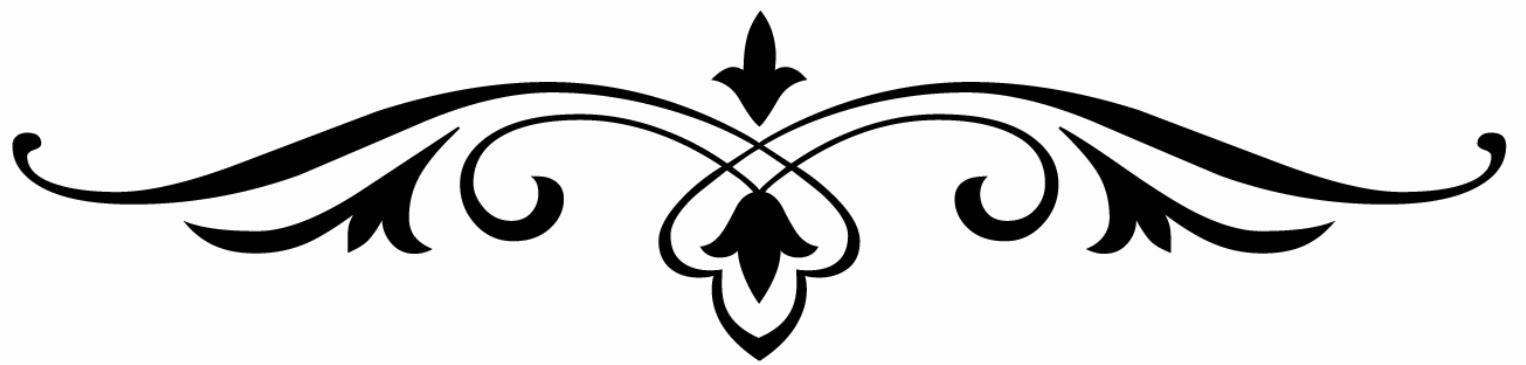
\includegraphics[scale=0.08]{end}\end{center}

\clearpage

\section{प्रश्नोत्तरमालिका}
\thispagestyle{empty}
\begin{enumerate}
\setlength\itemsep{-0.5em}
	\item को गुरुः~? अधिगततत्त्वः शिष्यहिताय उद्यतः सततम्~।
	\item कः शिष्यः~? भक्तिमान्~। 
	\item को हि जगद्गुरुः~। शम्भुः~।
	\item कः पण्डितः~? 
	विवेकी~।\footB\
	\item कः साधुः~? 
	सद्वृत्तः~।\footB\
	\item साधुबलं किम्~? 
	दैवम्~।\footB\
	\item दैवं किम्~? यत्सुकृतम्~।
	\item प्रत्यक्षदेवता का~? माता
	\item पूज्यो गुरुश्च कः~? 
	तातः~।\footB\
	\item कः सर्वदेवतात्मा~? विद्याकर्मान्वितो विप्रः~।
	\item का विद्या~? 
	या विमुक्तये~।\footB\
	\item किं कर्म~? 
	यत् चित्तशुद्धये~।\footB\
	\item का च परदेवतोक्ता~? चिच्छक्तिः~।
	\item कस्मै नमांसि देवाः कुर्वन्ति~? 
	दयाप्रधानाय~।\footB\
	\item कः पथ्यतरः~? 
	धर्मः~।\footB\
	\item कः शुचिरिह~? यस्य मानसं शुद्धम्~।
	\item किं विषमम्~? 
	अवधीरणा गुरुषु~।\footB\
	\item अवधीरणा क्व कार्या~? खल-परयोषित्-परधनेषु ।
	\item मदिरेव  मोहजनकः कः~? 
	स्नेहः~।\footB\
	\item का भववल्ली~? 
	तृष्णा~।\footB\
	\item किं गुरुताया मूलम्~? यदेतदप्रार्थनं नाम~।
	\item किं लाघवम्~? अधमतो याञ्चा~।
	\item को जागर्ति~? विवेकी~।
	\item का निद्रा~? मूढता जन्तोः~।
	\item नलिनीदलगतजलवत्तरलं किम्~? 
	यौवनं धनं चायुः~।\footB\
	\item के शशिकिरणसमाः? 
	सज्जना एव~।\footB\
	\item को नरकः~? परवशता~।\footB\
	\item किं सौख्यं~? 
	सर्वसङ्गविरतिर्या~।\footB\
	\item किं सत्यम्~? 
	भूतहितम्~।\footB\
	\item प्रियं किं प्राणिनाम्? 
	असवः~।\footB\
	\item कोऽनर्थफलः~? 
	मानः~।\footB\
	\item का सुखदा~? 
	साधुजनमैत्री~।\footB\
	\item किम् अन्नदायि~? अायुः ।
	\item सर्वव्यसनविनाशे को दक्षः~? 
	सर्वथा त्यागी~।\footB\
	\item किं चानर्घम्~? 
	यदवसरे दत्तम्~।\footB\
	\item आ मरणात्किं शल्यं~? प्रच्छन्नं यत्कृतं पापम्~।
	\item कुत्र विधेयो यत्नः~?विद्याभ्यासे सदौषधे दाने~।
	\item का प्रेयसी विधेया~? करुणा दीनेषु~,सज्जने मैत्री~।
	\item केन जितं जगदेतत्~? 
	सत्य-तितिक्षावता पुंसा~।\footB\ 
	\item कस्य वशे प्राणिगणः~? सत्य-प्रियभाषिणो विनीतस्य~।
	\item कोऽन्धः~? 
	योऽकार्यरतः~।\footB\
	\item को बधिरः~? यो हितानि न शृणोति~।
	\item को मूकः~? यः काले प्रियाणि वक्तुं न जानाति~।
	\item कः पङ्गुरिह  प्रथितः~? 
	व्रजति च यो वार्धके तीर्थम्~।\footB\
	\item चक्षुष्मन्तोऽप्यन्धाः के स्युः~? नास्तिका मनुजाः~।
	\item अन्धादिह को विशिष्यते~? 
	रागी~।\footB\
	\item के च दस्यवः~? विषयाः~।\footB\
	\item किं दानम्? 
	अनाकाङ्क्षम्~।\footB\
	\item किं मित्रम्~? यो निवारयति पापात्~।
	\item को राजा~? रञ्जनकृत् ~।
	\item कश्च श्वा ~? 
	नीचसेवकः।\footB\
	\item कोऽलङ्कारः~? शीलं~।
	\item किं तीर्थं मुख्यम्~? चित्तमलं यन्निवर्तयति ।
	\item को मृत्युः~? अवधानरहितत्वम् ।
	\item किं बीजं सर्वसुखानाम्~? पुण्यम् ।
	\item किं वाचां मण्डनम्~? सत्यम्~।
	\item किं विद्युद्विलसितचपलम्~? दुर्जनसंगतिः युवतयश्च~।
	\item चिन्तामणिरिव दुर्लभचतुष्कमिह किम्~? दानं प्रियवाक्सहितं, ज्ञानमगर्वं, क्षमान्वितं शौर्यम्, वित्तं त्यागसमेतम्~।
	\item किं शोच्यं~? 
	कार्पण्यं सति विभवे ~।\footB\
	\item किं प्रशस्तम्~? औदार्यम्~।
	\item कः कुलकमलदिनेशः~? सति गुणविभवेऽपि यो नम्रः~।
	\item कस्य वशे जगदेतत्~? प्रियहितवचनस्य  धर्मनिरतस्य~।
	\item कस्मै स्पृहयति  कमला~? 
	अनलसचित्ताय नीतिवृत्ताय~।\footB\
	\item कुत्र विधेयो वासः~? सज्जननिकटे~।
	\item रामादपि कः शूरः~? 
	स्मरशरनिहतो न यश्चलति~।\footB\
	\item किमहर्निशमनुचिन्त्यम्~? भगवच्चरणम्~।
	\item को हि न वाच्यः  सुधिया~? परदोषः अनृतञ्च~।
	\item प्राणादपि को रम्यः ~? कुलधर्मः साधुसङ्गश्च~।
	\item का कल्पलता लोके~? सच्छिष्याय अर्पिता विद्या~।
	\item कोऽक्षयवटवृक्षः स्यात्~? विधिवत् सत्पात्रदत्तदानम्~।
	\item कुत्र विषं~? दुष्टजने~।
	\item किमिहाशौचम्  भवेन्नॄणाम्~? ॠणम्~।
	\item किमभयमिह~? वैराग्यम् ~।
	\item भयमपि किं सर्वेषाम्~? वित्तमेव~।
	\item का दुर्लभा नराणाम्~?  हरिभक्तिः~।
	\item कः सर्वगुणविनाशकः~? लोभः~।
	\item पातकञ्च किम्~? हिंसा~।
	\item को हि भगवत्प्रियः स्यात्~? 
	यो अनुद्विग्नः अन्यं नोद्वेजयेत्~।\footB\
	\item कस्मात्सिद्धिः~? तपसः।
	\item कुतो बुद्धिः~? वृद्धोपसेवया~।
	\item के वृद्धाः~? ये धर्मतत्त्वज्ञाः~।
	\item संभावितस्य मरणादधिकं किम्~? दुर्यशः।
	\item को वर्धते~? विनीतः~।
	\item को वा हीयेत~? यो दृप्तः~।
	\item को न प्रत्येतव्यः~? ब्रूते यश्चानृतं शश्वत्~।
	\item कुत्रानृतेऽप्यपापम्~? यच्चोक्तं धर्मरक्षार्थम्~।
	\item को यज्ञः~? यः श्रुत्या विहितः श्रेयस्करो नॄणाम्~।
	\item किं भाग्यं देहवताम्~? आरोग्यम्~।
	\item किं दुष्करं नराणाम्~? यन्मनसो निग्रहः सततम्~।
	\item कस्य न शोकः~? यः स्यादक्रोधः~।
	\item किं सुखम्~? 
	तुष्टिः ~।\footB\
	\item क इन्द्रजालायते~? प्रपञ्चोऽयम्~।
	\item वपुषश्च पोषकं किम् ~? 
	प्रारब्धम्~।\footB\
	\item केषाम् अमोघवचनम्~? ये च पुनः सत्यमौनशमशीलाः~।
	\item त्वरितं किं कर्तव्यं विदुषाम्~? संसारसन्ततिच्छेदः |
	\item मोक्षश्च कः~? अविद्यास्तमयः।
	\item का चाविद्या~? यदात्मनोऽस्फूर्तिः~।
	\item किं मोक्षतरोर्बीजम्~? सम्यग्ज्ञानं क्रियासिद्धम्~।
	\item ज्ञानं कुतः~? शिवादेव~।
	\item कः सर्ववेदभूः~? ओम्~।\footB\
\end{enumerate}
\begin{center}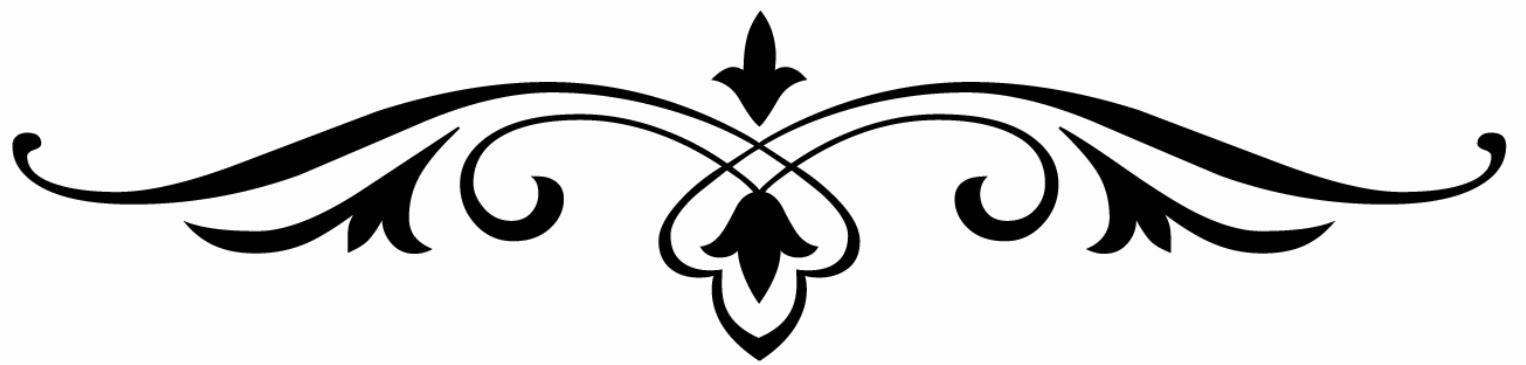
\includegraphics[scale=0.08]{end}\end{center}

\input Akara
   
\end{document}
